\documentclass[12pt,onecolumn,a4paper]{book}

%% 引用宏包 %%
\usepackage{ctex}
\usepackage{titlesec}
\usepackage{amsmath,amssymb,amsthm,multicol,siunitx,graphicx,enumitem,booktabs,appendix}
\usepackage{booktabs}
\usepackage{tabularx,subcaption,arydshln}
\usepackage{tikz}
\usepackage{arydshln}
\usetikzlibrary{calc}
\usetikzlibrary{positioning}
\usepackage[edges]{forest}
\usepackage{pgfplots}

\usetikzlibrary{matrix, positioning, arrows}
\usepackage{imakeidx}
\usepackage{hyperref}

\usepackage[most]{tcolorbox}
% 定义 block 环境
\newenvironment{block}[1]{
    \begin{tcolorbox}[colback=blue!5!white,colframe=blue!75!black,title=#1]
}{
    \end{tcolorbox}
}


%% 定义新定理 %%
\newtheorem*{example}{例}
\newtheorem*{lemma}{引理}
\newtheorem*{note}{注}

%% 设置初始编号 %%
\setcounter{section}{0}
\numberwithin{table}{subsection}
\numberwithin{equation}{subsection}

%% 设置超链接 %%
\hypersetup{
    hidelinks, % 取消红框
    colorlinks=true,
    linkcolor=blue,
    citecolor=black
}

%% BibTeX %%
\bibliographystyle{plain}
% \bibliography{}

%% 标题 %%
\title{电磁学}
\author{AnZrew}
\date{癸卯秋冬于清华园}

% \makeindex 

\begin{document}

\maketitle

\tableofcontents

\chapter{真空中的静电场}

\begin{block}{方程}
    \begin{align}
        \text{微分形式} \quad
         & \left\{
        \begin{aligned}
            \nabla \cdot \mathbf{E}  & = \frac{\rho}{\varepsilon_0} \\
            \nabla \times \mathbf{E} & = 0
        \end{aligned}
        \right.    \\
        \text{积分形式} \quad
         & \left\{
        \begin{aligned}
            \oint \mathbf{E} \cdot \mathrm{d} \mathbf{S} & = \frac{Q_{\text{inside}}}{\varepsilon_0} \\
            \oint \mathbf{E} \cdot \mathrm{d} \mathbf{l} & = 0
        \end{aligned}
        \right.
    \end{align}
\end{block}

\begin{block}{常数}
    \begin{align}
        \varepsilon_0 & = \SI{8.8542e-12}{\coulomb\squared\per\newton\per\meter\squared} \\
        k             & = \SI{8.9880e9}{\newton\meter\squared\per\coulomb\squared}
    \end{align}
\end{block}

\begin{block}{无穷大平板电场}
    \begin{align}
        \mathbf{E}(\mathbf{r}) & = \frac{\sigma}{2 \varepsilon_0} \hat{\mathbf{n}}
    \end{align}
\end{block}

\newpage

\section{电荷}

\subsection{量子性(Millikan实验)}

$$
    m = \frac{Q}{F} \frac{M}{z}
$$

\subsection{理想的点电荷}

用delta函数描述:

\begin{align}
    \rho(\mathbf{r}) & = q \delta(\mathbf{r} - \mathbf{r}_0)
\end{align}

\begin{note}
    \begin{enumerate}
        \item $\delta$函数的性质
              \begin{align}
                  \int_{-\infty}^{+\infty} \delta(x - x_0) \mathrm{d} x     & = 1      \\
                  \int_{-\infty}^{+\infty} f(x)\delta(x - x_0) \mathrm{d} x & = f(x_0)
              \end{align}
    \end{enumerate}
\end{note}

\subsection{电荷连续分布概率}

物质中电荷密度分布,可以近似为连续分布:

\begin{align}
    \rho(\mathbf{r}) & = \lim_{\Delta V \to 0} \frac{Q_{\text{inside}\Delta V}}{\Delta V} = \frac{\mathrm{d} Q}{\mathrm{d} V}
\end{align}

\subsection{对称性}

Dirac:正电子

\subsection{电荷守恒定律}

\begin{align}
    \frac{\partial \rho}{\partial t} + \nabla \cdot \mathbf{J} & = 0
\end{align}

其中$\mathbf{J}$为流场,$\mathbf{J} = \rho \mathbf{u}$。

\begin{proof}
    \begin{align}
        \frac{\partial}{\partial t} \int_{V} \rho \mathrm{d} V = - \oint_{S} \rho \mathbf{u} \cdot \mathrm{d} \mathbf{S} = - \int_{V} \nabla \cdot \mathbf{J} \mathrm{d} V
    \end{align}
    用物理的视角就是,电荷的变化率等于电荷流出的速率。
\end{proof}

\subsection{相对论不变性}

\section{Coulomb定律}

通过扭秤实验,可以得到电荷之间的相互作用力与距离的平方成反比。

\begin{align}
    \mathbf{F}_{12} & = \frac{1}{4 \pi \varepsilon_0} \frac{q_1 q_2}{\mathbf{r_{12}}^2} \hat{\mathbf{r}}_{12}
\end{align}

$\frac{1}{4 \pi \varepsilon_0}=k=\SI{8.9880e9}{\newton\meter\squared\per\coulomb\squared}$称为电磁力常数。

\section{电场与叠加原理}

\begin{align}
    \mathbf{F}_{12} & = \frac{q_1 q_2}{4 \pi \varepsilon_0} \frac{\mathbf{r_{1}}-\mathbf{r_{2}}}{\|\mathbf{r_{1}-\mathbf{r_{2}}}\|^3}
\end{align}

电场与电场强度(electric field and electric field intensity)定义为:

\begin{align}
    \mathbf{E}(\mathbf{r}) & = \frac{\mathbf{F}}{q}
\end{align}

其中$q$为静止的检验(点)电荷,$\mathbf{F}$为检验电荷受的电场力。单位为$\si{\newton\per\coulomb}= \si{\volt\per\meter}$。

场是一种近距相互作用。

有叠加原理(Superposition principle):

\begin{align}
    \mathbf{E}(\mathbf{r}) & = \sum_{i} \mathbf{E}_{i}(\mathbf{r})
\end{align}

\subsection{常见电场举例}

\begin{enumerate}
    \item 点电荷
          \begin{align}
              \mathbf{E}(\mathbf{r}) & = \frac{q}{4 \pi \varepsilon_0} \frac{\mathbf{r}-\mathbf{r_{0}}}{\|\mathbf{r}-\mathbf{r_{0}}\|^3}
          \end{align}
    \item 电偶极子
          \begin{align}
              \mathbf{E}(\mathbf{r}) & = \frac{1}{4 \pi \varepsilon_0} \frac{3(\mathbf{p} \cdot \hat{\mathbf{r}}) \hat{\mathbf{r}} - \mathbf{p}}{\|\mathbf{r}\|^3}
          \end{align}
          计算时利用Taylor展开,保留到二阶项。
    \item 连续体
          \begin{align}
              \mathbf{E}(\mathbf{r}) & = \frac{1}{4 \pi \varepsilon_0} \int_{V} \frac{\rho(\mathbf{r'})}{\|\mathbf{r}-\mathbf{r'}\|^3} (\mathbf{r}-\mathbf{r'}) \mathrm{d} V'
          \end{align}
          例如电荷均匀分的环形栅极:


\end{enumerate}

\section{Gauss定理}

\subsection{电场线}

电场线是电场的一种图像,它的定义为:

\begin{enumerate}
    \item 电场线的切线方向为电场强度的方向。
    \item 电场线的密度与电场强度的大小成正比。
    \item 电场线不会相交。
\end{enumerate}

\subsection{电通量}

我们认为电通量是通过该面的电场线的数量:

\begin{align}
    \|\mathbf{E}\| = \alpha \frac{\mathrm{d}N_\text{条数}}{\mathrm{d}S_{\bot}}
\end{align}

电通量定义为:

\begin{align}
    \Phi_{\mathbf{E}} & = \int_{S} \mathbf{E} \cdot \mathrm{d} \mathbf{S}
\end{align}

约定$\mathrm{d} \mathbf{S}$的方向为闭合曲面向外的法向。单位为$\si{\newton\meter\squared\per\coulomb}=\si{\volt\meter}$。

则有:

\begin{align}
    \Phi_{\mathbf{E}} & = \int_{S} \mathbf{E} \cdot \mathrm{d} \mathbf{S} = \int_{S} \|\mathbf{E}\| \theta \mathrm{d} S_{\bot} = \iint \alpha \mathrm{d} N = \alpha N
\end{align}

\subsection{Gauss定理}

在真空中的静电场内,通过任意闭合曲面的电通量,等于该曲面所包围电量的代数和除以真空介电常数。
\begin{align}
    \oint_{S} \mathbf{E} \cdot \mathrm{d} \mathbf{S} & = \frac{Q_{\text{inside}}}{\varepsilon_0}
\end{align}

从电力线的角度看是符合直觉的。

\begin{proof}
    \begin{align}
        \oint_{S} \mathbf{E} \cdot \mathrm{d} \mathbf{S} & = \oint_{S} \frac{1}{4 \pi \varepsilon_0} \frac{\rho(\mathbf{r'})}{\|\mathbf{r}-\mathbf{r'}\|^3} (\mathbf{r}-\mathbf{r'}) \cdot \mathrm{d} \mathbf{S} \\
                                                         & = \frac{1}{4 \pi \varepsilon_0} \int_{V} \rho(\mathbf{r'}) \mathrm{d} V'                                                                              \\
                                                         & = \frac{Q_{\text{inside}}}{\varepsilon_0}
    \end{align}
\end{proof}

\begin{note}
    \begin{enumerate}
        \item Gauss定理是平方反比律的必然结果;
        \item 电通量由S面内的电荷量的值决定, 与其分布无关;
        \item E是总场强,它由q内和q外共同决定;
        \item 高斯定理也适用于变化电场。
    \end{enumerate}
\end{note}

Gauss定理的微分形式:

\begin{align}
    \nabla \cdot \mathbf{E} & = \frac{\rho}{\varepsilon_0}
\end{align}

\begin{proof}
    \begin{align}
        \oint_{S} \mathbf{E} \cdot \mathrm{d} \mathbf{S} & = \int_{V} \nabla \cdot \mathbf{E} \mathrm{d} V                    \\
        = \frac{Q_{\text{inside}}}{\varepsilon_0}
                                                         & = \frac{1}{\varepsilon_0} \int_{V} \rho(\mathbf{r'}) \mathrm{d} V'
    \end{align}
\end{proof}

这是Maxwell方程组中的第一个方程。

\subsection{常见电场举例}

除了上面的叠加定理,可以取Gauss面分析问题。

\begin{enumerate}
    \item 均匀球
          \begin{align}
              \mathbf{E_\text{out}}(\mathbf{r}) & = \frac{1}{4 \pi \varepsilon_0} \frac{Q}{r^2} \hat{\mathbf{r}}                                                                          \\
              \mathbf{E_\text{in}}(\mathbf{r})  & =  \frac{1}{4 \pi \varepsilon_0} \frac{\frac{r^3}{R^3}Q}{r^2} \hat{\mathbf{r}} = \frac{1}{4 \pi \varepsilon_0} \frac{Q}{R^3} \mathbf{r}
          \end{align}
    \item 无穷大平板
          \begin{align}
              \mathbf{E}(\mathbf{r}) & = \frac{\sigma}{2 \varepsilon_0} \hat{\mathbf{n}}
          \end{align}
    \item 无穷长直线
          \begin{align}
              \mathbf{E}(\mathbf{r}) & = \frac{\lambda}{2 \pi \varepsilon_0} \frac{1}{r} \hat{\mathbf{r}}
          \end{align}
\end{enumerate}

\section{环路定理}

静电场的环量恒等于零,即对任意闭合路径 $L$ 有:

\begin{align}
    \oint_{L} \mathbf{E} \cdot \mathrm{d} \mathbf{l} & = 0
\end{align}

\begin{proof}
    \begin{align}
        \oint_{L} \mathbf{E} \cdot \mathrm{d} \mathbf{l} & = \oint_{L} \nabla \phi \cdot \mathrm{d} \mathbf{l}       \\
                                                         & = \oint_{L} \frac{\partial \phi}{\partial l} \mathrm{d} l \\
                                                         & = 0
    \end{align}
\end{proof}

\begin{note}
    \begin{enumerate}
        \item 电场力做功与路径无关,只与起点与终点的位置有关;
        \item 静电场沿任何闭合环路做功为零,是保守场;
        \item 静电场是一个无旋场,不会出现任何闭合的电场线;
        \item 环路定理是有心力场的必然结果。
    \end{enumerate}
\end{note}

环路定理的微分形式:

\begin{align}
    \nabla \times \mathbf{E} & = 0
\end{align}

这是因为有心力是保守的。

这是Maxwell方程组中的第二个方程(在静电场情况下)。

\subsection{电势}

旋度为零在数学上意味着是一个势函数的梯度,即:

\begin{align}
    \mathbf{E} & = - \nabla \phi
\end{align}

$\phi$称为电势,单位为伏特(V)。

\begin{align}
    \phi(\mathbf{r}) & = - \int_{\mathbf{r_0}}^{\mathbf{r}} \mathbf{E} \cdot \mathrm{d} \mathbf{l}
\end{align}

我们定义无穷远处电势为零。

\section{Coulomb定律+叠加原理与Gauss定理+环路定理的等价性}

\subsection{立体角}

\begin{align}
    \mathrm{d}\Omega & = \frac{\mathrm{d} S_{\bot}}{r^2}
\end{align}

对于一个闭合曲面,有:

\begin{align}
    \oint_{S} \mathrm{d} \Omega & = 4 \pi & (\text{if } \mathbf{r} \text{ is inside} ) \\
                                & = 0     & (\text{if } \mathbf{r} \text{ is outside})
\end{align}

\subsection{等价性说明}

\subsubsection{Coulomb定律+叠加原理 $\Rightarrow$ Gauss定理+环路定理}

\begin{proof}
    对一个点电荷,有:
    \begin{align}
        \oint_{S} \mathbf{E} \cdot \mathrm{d} \mathbf{S} & = \oint_{S} \frac{q}{4 \pi \varepsilon_0} \frac{\hat{\mathbf{r}}\hat{\mathbf{n}}}{\|\mathbf{r}\|^2} \cdot \mathrm{d} \mathbf{S} \\
                                                         & = \frac{1}{4 \pi \varepsilon_0} \oint_{S} \mathrm{d} \Omega                                                                     \\
                                                         & = \frac{q_{\text{inside}}}{\varepsilon_0}
    \end{align}

    \begin{align}
        \oint_{L} \mathbf{E} \cdot \mathrm{d} \mathbf{l} & = \oint_{L} f(r)\mathbf{r} \mathrm{d} \mathbf{r} \\
                                                         & = \oint_{L} f(r)r \mathrm{d} r                   \\
                                                         & = 0
    \end{align}
    叠加可得。
\end{proof}

\subsubsection{Gauss定理+环路定理 $\Rightarrow$ Coulomb定律+叠加原理}

\begin{proof}
    前两个方程可得:

    \begin{align}
        \nabla \cdot \mathbf{E}  & = \frac{\rho}{\varepsilon_0} \\
        \nabla \times \mathbf{E} & = 0
    \end{align}

    这意味着$\mathbf{E}$是一个保守场,即存在势函数$\phi$,使得:

    \begin{align}
        \mathbf{E} & = - \nabla \phi
    \end{align}

    从而有Poisson方程:

    \begin{align}
        \nabla^2 \phi & = - \frac{\rho}{\varepsilon_0}
    \end{align}

    对于点源,有Green函数:

    \begin{align}
        \phi(\mathbf{r}) & = \frac{1}{4 \pi \varepsilon_0} \frac{q}{\|\mathbf{r}-\mathbf{r_0}\|}
    \end{align}

    从而有:

    \begin{align}
        \mathbf{E}(\mathbf{r}) & = \frac{1}{4 \pi \varepsilon_0} \frac{q}{\|\mathbf{r}-\mathbf{r_0}\|^3} (\mathbf{r}-\mathbf{r_0})
    \end{align}

\end{proof}

\section{总结}

静电场主要是三个物理量的关系:电荷密度$\rho$,电场强度$\mathbf{E}$,电势$\phi$。由Maxwell的静电场方程给出:

\begin{align}
    \nabla \cdot \mathbf{E}  & = \frac{\rho}{\varepsilon_0} \\
    \nabla \times \mathbf{E} & = 0                          \\
    \mathbf{E}               & = - \nabla \phi
\end{align}

\chapter{静电场中的导体与电介质}

\begin{block}{方程}
    \begin{align}
        \quad
        \text{边值关系} \quad & \left\{
        \begin{aligned}
            \nabla \cdot \mathbf{D}  & = \rho_0                                & \text{Gauss定理} \\
            \nabla \times \mathbf{E} & = 0                                     & \text{环路定理}    \\
            \mathbf{D}               & = \varepsilon_0 \mathbf{E} + \mathbf{P} & \text{物质方程}    \\
        \end{aligned}
        \right.                     \\
        \text{边值关系} \quad
                          & \left\{
        \begin{aligned}
            \mathbf{D}_{1n}                                 & = \mathbf{D}_{2n}                                 \\
            \mathbf{E}_{1t}                                 & = \mathbf{E}_{2t}                                 \\
            \phi_1                                          & =   \phi_2                                        \\
            \varepsilon_1\frac{\partial \phi_1}{\partial n} & = \varepsilon_2\frac{\partial \phi_2}{\partial n}
        \end{aligned}
        \right.
    \end{align}
\end{block}

\begin{block}{电介质}
    \begin{align}
                   & \text{极化电介质 = 真空 + 极化面电荷$\sigma'$ + 极化体电荷$\rho'$}                                                       \\
        \sigma'    & = \mathbf{P} \cdot \hat{\mathbf{n}}                                                                     \\
        \rho'      & = -\nabla \cdot \mathbf{P}                                                                              \\
        \mathbf{P} & = \chi_e \varepsilon_0 \mathbf{E}                                                                       \\
        \mathbf{D} & = \varepsilon_0 (1+\chi_e) \mathbf{E} = \varepsilon_0 \varepsilon_r \mathbf{E} = \varepsilon \mathbf{E}
    \end{align}
\end{block}

\begin{block}{电偶极子}
    \begin{align}
        \mathbf{E} & = \frac{1}{4 \pi \varepsilon_0} \frac{3(\mathbf{p} \cdot \hat{\mathbf{r}}) \hat{\mathbf{r}} - \mathbf{p}}{\|\mathbf{r}\|^3} \\
        \phi       & = \frac{1}{4 \pi \varepsilon_0} \frac{\mathbf{p} \cdot \hat{\mathbf{r}}}{\|\mathbf{r}\|^2}                                  \\
        \mathbf{M} & = \mathbf{p} \times \mathbf{E}                                                                                              \\
        \mathbf{F} & = \mathbf{p} \cdot \nabla \mathbf{E}
    \end{align}
\end{block}

\newpage

\section{物质的电性质}

\subsection{物质的场}

物质中的场是指宏观场。选微观足够大,宏观足够小的体积对微观场(局域场 Local Field)取平均得到宏观场。该宏观场满足Maxwell方程组。

\begin{align}
    \mathbf{E} = \langle \mathbf{E}_\text{Local}\rangle
\end{align}

\subsection{物质的电性质}

物质根据电性质分为绝缘体、半导体、导体、超导体,他们的区别在于电阻率$\rho$。

\section{静电场中的导体}

\subsection{静电场中的导体的性质}

\begin{enumerate}
    \item 导体内部的电场为零。

          导体内部有自由载流子,达到静电平衡时,自由载流子不再运动。外部电场和感应电场平衡。
    \item 导体表面的电场垂直于表面,表面是等势面。

          导体表面的电场与表面平行,否则会有电场力使得自由载流子运动。

          \begin{figure}[ht]
              \centering


              \tikzset{every picture/.style={line width=0.75pt}} %set default line width to 0.75pt        

              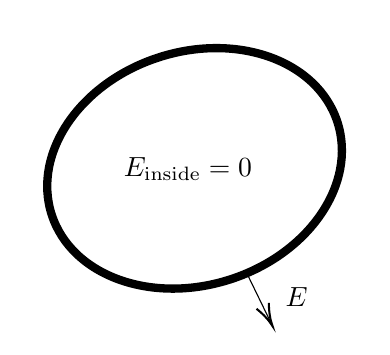
\begin{tikzpicture}[x=0.75pt,y=0.75pt,yscale=-1,xscale=1]
                  %uncomment if require: \path (0,300); %set diagram left start at 0, and has height of 300

                  %Shape: Ellipse [id:dp5032785818104535] 
                  \draw  [line width=3]  (148.53,159.15) .. controls (138.95,129.63) and (162,95.7) .. (200.01,83.37) .. controls (238.02,71.03) and (276.6,84.96) .. (286.18,114.48) .. controls (295.76,143.99) and (272.71,177.92) .. (234.7,190.26) .. controls (196.69,202.59) and (158.11,188.66) .. (148.53,159.15) -- cycle ;
                  %Straight Lines [id:da9435368832910616] 
                  \draw    (242.95,188.2) -- (254.08,211.06) ;
                  \draw [shift={(254.95,212.86)}, rotate = 244.06] [color={rgb, 255:red, 0; green, 0; blue, 0 }  ][line width=0.75]    (10.93,-3.29) .. controls (6.95,-1.4) and (3.31,-0.3) .. (0,0) .. controls (3.31,0.3) and (6.95,1.4) .. (10.93,3.29)   ;

                  % Text Node
                  \draw (260,193) node [anchor=north west][inner sep=0.75pt]   [align=left] {$E$};
                  % Text Node
                  \draw (182,130.33) node [anchor=north west][inner sep=0.75pt]   [align=left] {$E_\text{inside}=0$};


              \end{tikzpicture}
              \caption{导体表面的电场}
          \end{figure}
    \item 导体表面的电荷分布在表面。

          $\sigma$可不为零,但内部$\rho$必为零。这是因为Maxwell方程组的第一式:

          \begin{align}
              \nabla \cdot \mathbf{E} & = 0 = \frac{\rho}{\varepsilon_0}
          \end{align}

    \item 对于空腔导体:

          \begin{figure}[ht]
              \centering

              \tikzset{every picture/.style={line width=0.75pt}} %set default line width to 0.75pt        

              \begin{tikzpicture}[x=0.75pt,y=0.75pt,yscale=-1,xscale=1]
                  %uncomment if require: \path (0,300); %set diagram left start at 0, and has height of 300

                  %Shape: Ellipse [id:dp5032785818104535] 
                  \draw  [line width=3]  (148.53,159.15) .. controls (138.95,129.63) and (162,95.7) .. (200.01,83.37) .. controls (238.02,71.03) and (276.6,84.96) .. (286.18,114.48) .. controls (295.76,143.99) and (272.71,177.92) .. (234.7,190.26) .. controls (196.69,202.59) and (158.11,188.66) .. (148.53,159.15) -- cycle ;
                  %Shape: Ellipse [id:dp20671837862395814] 
                  \draw  [line width=3]  (164.47,129.28) .. controls (169.85,106.28) and (197.38,93.06) .. (225.96,99.74) .. controls (254.54,106.43) and (273.34,130.49) .. (267.96,153.49) .. controls (262.58,176.49) and (235.05,189.71) .. (206.47,183.02) .. controls (177.89,176.34) and (159.09,152.27) .. (164.47,129.28) -- cycle ;

                  % Text Node
                  \draw (274.67,159) node [anchor=north west][inner sep=0.75pt]   [align=left] {$\displaystyle \sigma_\text{外表面}$};
                  % Text Node
                  \draw (244,93) node [anchor=north west][inner sep=0.75pt]   [align=left] {$\displaystyle E_\text{导体内}=0$};
                  % Text Node
                  \draw (198,100.33) node [anchor=north west][inner sep=0.75pt]   [align=left] {$\displaystyle \sigma_\text{内表面} $};
                  % Text Node
                  \draw (178,133.67) node [anchor=north west][inner sep=0.75pt]   [align=left] {$\displaystyle E_\text{内}e=0$};


              \end{tikzpicture}
              \caption{空腔导体}
          \end{figure}

          在导体内部取Gauss面,由于导体内部电场强度恒为0,可以得到$\sigma_\text{内表面}=0$。$\sigma_\text{外表面}$可能不为零。

          又由于电势满足Laplace方程:

          \begin{align}
              \nabla^2 \phi = 0
          \end{align}

          可以得到$\phi$在导体内部恒为常数,即$E_\text{内}=0$。

          如果空腔内部有电荷,则有内表面电荷不为0,由Gauss定理:

          \begin{align}
              \oint \sigma_\text{内表面} \mathrm{d} S & = - Q_\text{inside}
          \end{align}

          外表面电荷为:

          \begin{align}
              \oint \sigma_\text{外表面} \mathrm{d} S & = Q_\text{inside}
          \end{align}

          这时空腔内部的电场强度不为零,但是导体内部的电场强度仍然为零(感应电荷和内部电荷电场的共同作用)。

    \item 表面场强与面电荷密度的关系

          取一个贴近表面的小Gauss面,内部电场强度为0,有:
          \begin{align}
              \mathbf{E}_\text{表面} = \frac{\sigma}{\varepsilon_0}\hat{\mathbf{n}}
          \end{align}

          其中面积微元表面的电荷(无穷大平面)贡献$\frac{\sigma}{2\varepsilon_0}$,剩余的$\frac{\sigma}{2\varepsilon_0}$由面积微元外电荷贡献。

    \item 表面电荷分布与曲率的关系

          假设两个导体球相距无限远,导线相连,电荷量、面电荷密度和半径分别为$Q,q;\Sigma,\sigma;R,r$。二者电势相等则有:

          \begin{align}
              \frac{Q}{4\pi\varepsilon_0 R} = \frac{q}{4\pi\varepsilon_0 r}
          \end{align}

          从而:

          \begin{align}
              \frac{\Sigma}{\sigma} = \frac{r}{R}
          \end{align}

          这表示孤立导体表面曲率大处面电荷密度也大,但不存在单一函数关系。

          尖端放电(point discharge):带电的尖端电场强,使附近的空气电离,因而产生放电。
\end{enumerate}

\begin{example}
    面电荷密度为$\sigma_0$的均匀带电大平板旁,平行放置一大的不带电导体平板。求导体板两表面的面电荷密度。

    \begin{figure}[ht]
        \centering


        \tikzset{every picture/.style={line width=0.75pt}} %set default line width to 0.75pt        

        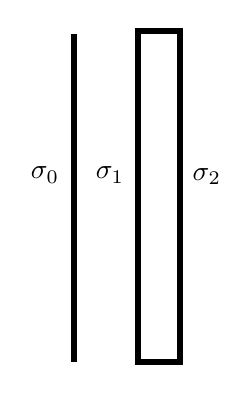
\begin{tikzpicture}[x=0.75pt,y=0.75pt,yscale=-1,xscale=1]
            %uncomment if require: \path (0,300); %set diagram left start at 0, and has height of 300

            %Straight Lines [id:da46092774428263117] 
            \draw [line width=2.25]    (131.33,53.77) -- (131.33,212) ;
            %Shape: Rectangle [id:dp24967145703562155] 
            \draw  [line width=2.25]  (162.29,52.33) -- (182.29,52.33) -- (182.29,211.77) -- (162.29,211.77) -- cycle ;

            % Text Node
            \draw (140.67,116.67) node [anchor=north west][inner sep=0.75pt]   [align=left] {$\displaystyle \sigma _{1}$};
            % Text Node
            \draw (187.33,117.33) node [anchor=north west][inner sep=0.75pt]   [align=left] {$\displaystyle \sigma _{2}$};
            % Text Node
            \draw (109.33,116.67) node [anchor=north west][inner sep=0.75pt]   [align=left] {$\displaystyle \sigma _{0}$};


        \end{tikzpicture}
        \caption{题图}
    \end{figure}

    电荷守恒:

    \begin{align}
        \sigma_1 + \sigma_2=0
    \end{align}

    导体内部电场强度为零,有:

    \begin{align}
        E_0+E_1-E_2                                                                                  & =0 \\
        \frac{\sigma_0}{\varepsilon_0}+\frac{\sigma_1}{\varepsilon_0}-\frac{\sigma_2}{\varepsilon_0} & =0
    \end{align}

    解得:

    \begin{align}
        \sigma_1 & = -\frac{\sigma_0}{2} \\
        \sigma_2 & = \frac{\sigma_0}{2}
    \end{align}

    如果右侧导体棒接地,由于无穷远和导体表面电势都为0,导体板右侧电场强度应为0,故电荷守恒式变为:

    \begin{align}
        \frac{\sigma_0}{\varepsilon_0}+\frac{\sigma_1}{\varepsilon_0}+\frac{\sigma_2}{\varepsilon_0} & =0
    \end{align}

    剩下的导体内部电场强度为零不变。解得:

    \begin{align}
        \sigma_1 & = -\sigma_0 \\
        \sigma_2 & = 0
    \end{align}
\end{example}

\subsection{静电唯一性定理}

\[
    \text{唯一性定理}\left\{
    \begin{array}{l}
        \text{给定电荷分布} \\
        \text{边界条件} \left\{
        \begin{array}{l}
            \text{第一类:边界电势分布【Dirichlet】}       \\
            \text{第二类:边界等电势,并给定电通量/电量【Neuman】} \\
            \text{第三类:混合边界条件}
        \end{array}
        \right.
    \end{array}
    \right.
\]

满足电荷分布和边界条件的电场是唯一的。

我们从物理和数学两个角度出发:

\subsubsection{物理角度}

\begin{lemma}[Lemma1]
    在无电荷的空间里电势不可能有极大值或极小值。

    \begin{proof}
        假设在某点有极大值,则在该点的邻域内取Gauss面,得到矛盾。

        或者又调和函数的性质,边界不可能取到最值。
    \end{proof}
\end{lemma}

\begin{lemma}[Lemma2]
    该空间中,若所有导体电势为零,则导体以外空间电势处处为零。

    \begin{proof}
        电势在无电荷空间连续分布,若空间有电势大于0(或小于0)的点,而边界上又处处等于0,在空间必出现电势的极大(或极小)值,这违背上一条引理。
    \end{proof}
\end{lemma}

可以得到一条推论:

\begin{lemma}[推论]
    若在完全由导体所包围的空间里各导体电势都相等(设为$U_0$),则空间电势等于常量$U_0$。
\end{lemma}

\begin{lemma}[Lemma3]
    若所有导体都不带电,则各导体的电势都相等。

    \begin{proof}
        如果存在最大的电势$U_0$,则在该点的邻域内取Gauss面,得到矛盾。
    \end{proof}
\end{lemma}

如果在给定电荷分布和边界条件的情况下,电势不唯一,电势设为$\phi_1(\mathbf{r}),\phi_2(\mathbf{r})$。记$\phi(\mathbf{r})=\phi_1(\mathbf{r})-\phi_2(\mathbf{r})$。

两类边界条件是:

\textbf{第一类【Dirichlet】:边界$S$上$\phi_i$确定}

\begin{align}
    \phi(\mathbf{r}) |_S & = 0
\end{align}

根据引理2,有:

\begin{align}
    \phi(\mathbf{r}) & = 0
\end{align}

这意味着唯一性:$\phi_1(\mathbf{r})=\phi_2(\mathbf{r})$。

\textbf{第二类【Neuman】:边界上$\frac{\partial \phi}{\partial n_i}$确定}

\begin{align}
    \oint \mathbf{E} \cdot \mathrm{d} \mathbf{S} & = \oint - \nabla \phi \mathrm{d} \mathbf{S}                     \\
                                                 & = \oint - \frac{\partial \phi}{\partial n_i} \mathrm{d} S_i = 0
\end{align}

其中:

\begin{align}
    \frac{\partial \phi}{\partial n_i}|_S=q(\mathbf{r})
\end{align}

表示的是边界上的电荷分布。从而做差后的$\phi$满足边界不带电。根据引理3:

\begin{align}
    \nabla \phi(\mathbf{r}) & = 0
\end{align}

这意味着唯一性:$\phi_1(\mathbf{r})=\phi_2(\mathbf{r})+C$,其中$C$为常数。

\subsubsection{数学角度}

我们考察这样一个式子:

\begin{align}
    \nabla(\phi \nabla \phi) & = \nabla \phi \cdot \nabla \phi + \phi \nabla^2 \phi
\end{align}

在无电荷的空间里,$\nabla^2 \phi = 0$,则:

\begin{align}
    \nabla(\phi \nabla \phi) & = |\nabla \phi|^2
\end{align}

从而:

\begin{align}
    \int \nabla(\phi \nabla \phi) \mathrm{d} V & = \oint \phi \nabla \phi \cdot \mathrm{d} \mathbf{S} \\
                                               & = \int |\nabla \phi|^2 \mathrm{d} V \geqslant 0
\end{align}

\begin{note}
    该式的物理含义:电荷系中的能量(电势$\times$电量)$\oint \phi \nabla \phi \cdot \mathrm{d} \mathbf{S}$=无电荷空间中的能量$\int |\nabla \phi|^2 \mathrm{d} V$。
\end{note}

根据这个式子,结合边界条件:

\begin{align}
    \oint \phi \nabla \phi \cdot \mathrm{d} \mathbf{S} = \int |\nabla \phi|^2 \mathrm{d} V & = 0
\end{align}

可知:

\begin{align}
    \nabla \phi & = 0
\end{align}

这就是唯一性。

\subsection{静电屏蔽}

\subsubsection{壳内域}

若$q_\text{内}$给定,则有方程:

\begin{align}
    q_\text{$S_\text{内}$}                        & = -q_\text{内}                      \\
    \oint \mathbf{E} \cdot \mathrm{d} \mathbf{S} & = \frac{q_\text{内}}{\varepsilon_0}
\end{align}


\begin{figure}[ht]
    \centering
    \includegraphics[scale=0.2]{pic/2.2.3.png}
    \caption{静电屏蔽}
\end{figure}

这符合唯一性定理的第二类边界条件。从而无论$q_\text{外}$如何变化,$\mathbf{E}_\text{内}$不变。

\textbf{封闭导体壳屏蔽了壳外电荷对壳内的影响。}

\subsubsection{壳外域}

若$q_\text{外}$给定,则有方程:

\begin{align}
    q_\text{$S_\text{外}$}                        & = q_\text{外}                       \\
    \oint \mathbf{E} \cdot \mathrm{d} \mathbf{S} & = \frac{q_\text{内}}{\varepsilon_0} \\
    \phi_\infty                                  & = 0
\end{align}

这符合唯一性定理的第三类边界条件。只要$q_\text{内}$不变化,位置不固定,$\mathbf{E}_\text{外}$不唯一确定。

\textbf{封闭导体壳部分屏蔽了壳内电荷对壳外的影响。}
\subsubsection{导体壳接地}

域内有方程:

\begin{align}
     & \text{$q_\text{内}$分布给定}                                     \\
     & \phi_\text{$S_\text{内}$}                                = 0
\end{align}

从而$\mathbf{E}_\text{内}$与$q_\text{外}$无关。

域外有方程:

\begin{align}
     & \text{$q_\text{外}$分布给定}                                     \\
     & \phi_\text{$S_\text{外}$}                                = 0
     & \phi_\infty                                = 0
\end{align}

从而$\mathbf{E}_\text{外}$与$q_\text{内}$无关。

\textbf{封闭导体壳完全屏蔽了内外场。}

\subsection{电像法}

根据静电唯一性定理,我们可以通过构造电像来求解静电场问题。

\begin{example}
    无限大均匀带电平面,距离为$d$处有一点电荷$q$。

    \begin{figure}[ht]
        \centering
        \includegraphics[scale=0.2]{pic/2.2.4.1.png}
        \caption{题图}
    \end{figure}

    在对称处找一个电荷相反的点电荷,使得电势在无穷远处为零。等效成电偶极子。
\end{example}

\begin{example}
    一个半径为R的金属球,距离球心为$d$处有一点电荷$q$。

    \begin{figure}[ht]
        \centering


        \tikzset{every picture/.style={line width=0.75pt}} %set default line width to 0.75pt        

        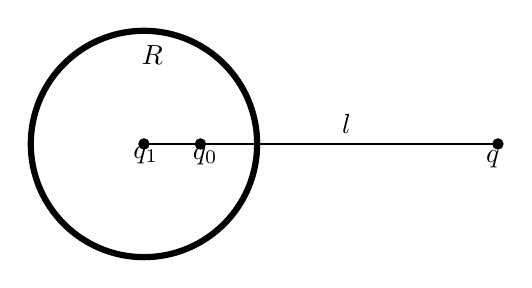
\begin{tikzpicture}[x=0.75pt,y=0.75pt,yscale=-1,xscale=1]
            %uncomment if require: \path (0,300); %set diagram left start at 0, and has height of 300

            %Shape: Circle [id:dp0355540611559928] 
            \draw  [line width=2.25]  (125.23,130.86) .. controls (125.23,100.75) and (149.64,76.33) .. (179.76,76.33) .. controls (209.87,76.33) and (234.29,100.75) .. (234.29,130.86) .. controls (234.29,160.97) and (209.87,185.39) .. (179.76,185.39) .. controls (149.64,185.39) and (125.23,160.97) .. (125.23,130.86) -- cycle ;
            %Straight Lines [id:da12683322984367473] 
            \draw    (179.76,130.86) -- (350.29,130.86) ;
            %Shape: Circle [id:dp5750047457677756] 
            \draw  [fill={rgb, 255:red, 0; green, 0; blue, 0 }  ,fill opacity=1 ] (347.81,130.86) .. controls (347.81,129.49) and (348.92,128.38) .. (350.29,128.38) .. controls (351.65,128.38) and (352.76,129.49) .. (352.76,130.86) .. controls (352.76,132.23) and (351.65,133.34) .. (350.29,133.34) .. controls (348.92,133.34) and (347.81,132.23) .. (347.81,130.86) -- cycle ;
            %Shape: Circle [id:dp08344717108862776] 
            \draw  [fill={rgb, 255:red, 0; green, 0; blue, 0 }  ,fill opacity=1 ] (177.28,130.86) .. controls (177.28,129.49) and (178.39,128.38) .. (179.76,128.38) .. controls (181.13,128.38) and (182.24,129.49) .. (182.24,130.86) .. controls (182.24,132.23) and (181.13,133.34) .. (179.76,133.34) .. controls (178.39,133.34) and (177.28,132.23) .. (177.28,130.86) -- cycle ;
            %Shape: Circle [id:dp23267069968229026] 
            \draw  [fill={rgb, 255:red, 0; green, 0; blue, 0 }  ,fill opacity=1 ] (204.48,130.86) .. controls (204.48,129.49) and (205.58,128.38) .. (206.95,128.38) .. controls (208.32,128.38) and (209.43,129.49) .. (209.43,130.86) .. controls (209.43,132.23) and (208.32,133.34) .. (206.95,133.34) .. controls (205.58,133.34) and (204.48,132.23) .. (204.48,130.86) -- cycle ;

            % Text Node
            \draw (177.33,82) node [anchor=north west][inner sep=0.75pt]   [align=left] {$\displaystyle R$};
            % Text Node
            \draw (202,131.33) node [anchor=north west][inner sep=0.75pt]   [align=left] {$\displaystyle q_{0}$};
            % Text Node
            \draw (173.33,130.67) node [anchor=north west][inner sep=0.75pt]   [align=left] {$\displaystyle q_{1}$};
            % Text Node
            \draw (343.33,132.67) node [anchor=north west][inner sep=0.75pt]   [align=left] {$\displaystyle q$};
            % Text Node
            \draw (274,115.33) node [anchor=north west][inner sep=0.75pt]   [align=left] {$\displaystyle l$};


        \end{tikzpicture}

        \caption{题图}
    \end{figure}

    根据等势面将球等效成$q_0$,由Apollonius圆可知:

    \begin{align}
        q_0 & = -\frac{qR}{l} \\
        d   & = \frac{R^2}{l}
    \end{align}

    为了平衡电荷,球上有电荷$q_1$,有:

    \begin{align}
        q_1 & = \frac{qR}{l} \\
    \end{align}
\end{example}

\section{静电场对物质的作用}

静电场对物质的作用本质上是电场对物质内部电荷的作用:

导体是电场对自由电荷的作用,可简化为点电荷;绝缘体是电场对极化电荷的作用,可简化为偶极子。

\textbf{电偶极子在电场内会受到力矩:}

\begin{align}
    \mathbf{M} & = \mathbf{r}_+ \times \mathbf{F}(\mathbf{r}_+) + \mathbf{r}_- \times \mathbf{F}(\mathbf{r}_-) \\
               & = q \mathbf{l} \times \frac{1}{2}(\mathbf{E}(\mathbf{r}_+)+\mathbf{E}(\mathbf{r}_-) )         \\
               & = \mathbf{p} \times \mathbf{E}(\mathbf{r})
\end{align}

\textbf{电偶极子在电场内会受到梯度力:}

\begin{align}
    \mathbf{F} & = \mathbf{F}(\mathbf{r}_+) - \mathbf{F}(\mathbf{r}_-)    \\
               & = q (\mathbf{E}(\mathbf{r}_+) -\mathbf{E}(\mathbf{r}_-)) \\
               & = q \mathbf{l} \cdot \nabla \mathbf{E}(\mathbf{r})       \\
               & = \mathbf{p} \cdot \nabla \mathbf{E}(\mathbf{r})
\end{align}

用到了全微分和梯度的关系:

\begin{align}
    \mathrm{d} \mathbf{E} & = \nabla \mathbf{E} \cdot \mathrm{d} \mathbf{r}
\end{align}

\section{电容}

对一个半径为$R$的孤立导体球,带电量为$Q$,电势为$U$:

\begin{align}
    U & = \frac{Q}{4\pi\varepsilon_0 R}
\end{align}

可知$Q$与$U$成正比,比例系数为$C$,称为电容,反应出导体球储存电荷的能力。单位是$F=CV$。

\begin{align}
    C & = \frac{Q}{U}
\end{align}

静电唯一性定理保证任意形状孤立导体电势与电量成正的线性关系。对任意形状的一对带等量异号电荷的导体,线性关系仍然成立。

\subsection{一些常见的电容}

\begin{enumerate}
    \item 平行板电容器(自屏蔽电容器)

          两板面积为$S$,距离为$d$,板上电荷量为$Q$,则:

          \begin{align}
              U & = \frac{Q}{\varepsilon_0 S}               \\
              C & = \frac{Q}{U} = \frac{\varepsilon_0 S}{d}
          \end{align}


    \item 球形电容器(自屏蔽电容器)

          内外半径分别为$R_1,R_2$,内外球面电荷量分别为$+Q,-Q$,则:

          \begin{align}
              U & = \frac{Q}{4\pi\varepsilon_0 R_1} - \frac{Q}{4\pi\varepsilon_0 R_2} \\
              C & = \frac{Q}{U} = \frac{4\pi\varepsilon_0 R_1 R_2}{R_2-R_1}
          \end{align}


    \item 圆柱形电容器(自屏蔽电容器)

          内外半径分别为$R_1,R_2$,高度为$h$,内外柱面电荷量分别为$+Q,-Q$,则:

          \begin{align}
              U & = \frac{Q}{2\pi\varepsilon_0 h} \ln \frac{R_2}{R_1}             \\
              C & = \frac{Q}{U} = \frac{2\pi\varepsilon_0 h}{\ln \frac{R_2}{R_1}}
          \end{align}

\end{enumerate}

\subsection{电容的串并联}

\begin{enumerate}
    \item 串联

          \begin{align}
              C & = \frac{Q}{U} = \frac{Q}{U_1+U_2} = \frac{Q}{Q/C_1+Q/C_2} \\
                & = \frac{1}{\frac{1}{C_1}+\frac{1}{C_2}}
          \end{align}

    \item 并联

          \begin{align}
              C & = \frac{Q}{U} = \frac{Q}{U_1} = \frac{Q}{U_2} \\
                & = C_1+C_2
          \end{align}
\end{enumerate}

\section{静电场中的电介质}

\subsection{多级展开与电介质的偶极子模型}

将势能函数在$\mathbf{r}_0$处展开:

\begin{align}
    \phi(\mathbf{r}) & = \frac{1}{4 \pi \varepsilon_0} \int \frac{\rho(\mathbf{r}')}{|\mathbf{r}-\mathbf{r}'|} \mathrm{d} V'                                                                                                                                                                         \\
                     & = \frac{1}{4 \pi \varepsilon_0} \frac{q}{|\mathbf{r}_0 |} + \frac{1}{4 \pi \varepsilon_0} \frac{\mathbf{p} \cdot \hat{\mathbf{r}_0}}{|\mathbf{r}_0 |^2} + \frac{1}{4 \pi \varepsilon_0} \frac{\hat{\mathbf{r}_0}^T \mathbf{Q} \hat{\mathbf{r}_0}}{|\mathbf{r}_0 |^3} + \cdots
\end{align}

其中:

\begin{align}
    \mathbf{p} & = \int \rho(\mathbf{r}') \mathbf{r}' \mathrm{d} V'                                  \\
    \mathbf{Q} & = \int \rho(\mathbf{r}') (3\mathbf{r}' \mathbf{r}' - \mathbf{I} r'^2) \mathrm{d} V'
\end{align}

是电荷分布的一阶和二阶矩,分别称为电偶极矩和电四极矩,是矢量和二阶张量。

我们认为电介质被外电场极化后可以等效为电偶极子,即:

\begin{align}
    \phi(\mathbf{r}) & =\frac{1}{4 \pi \varepsilon_0} \frac{\mathbf{p} \cdot \hat{\mathbf{r}_0}}{|\mathbf{r}_0 |^2}
\end{align}

\subsection{极化强度矢量}

电介质在电场中是下图的图景:

\begin{figure}[ht]
    \centering
    \includegraphics[scale=0.2]{pic/2.5.1.png}
    \caption{电介质在电场中的图景}
\end{figure}

在宏观足够小,微观足够大定义。(宏观场)

\begin{align}
    \mathbf{P} & = \lim_{\mathrm{d} V \rightarrow 0} \frac{\sum \mathbf{p}_\text{分子}}{\mathrm{d} V}
\end{align}

电极化矢量的量纲与面电荷密度相同,单位是$\mathrm{C/m^2}$。

\begin{align}
    \text{极化电介质 = 真空 + 极化面电荷$\sigma'$ + 极化体电荷$\rho'$}
\end{align}

\subsubsection{极化面电荷}

\begin{align}
    Q_\text{极化} & = q n \Delta V                       \\
                & = n \Delta S l q                     \\
                & = n p \Delta S                       \\
                & = \mathbf{P} \cdot \Delta \mathbf{S}
\end{align}

其中$n$是单位体积内的分子数。

从而极化面电荷密度:

\begin{align}
    \sigma' & = \frac{Q_\text{极化}}{\Delta S} = \mathbf{P} \cdot \hat{\mathbf{n}}
\end{align}

\subsubsection{极化体电荷}

在非均匀极化的情况下,极化体电荷密度:

\begin{align}
    \rho' & = \frac{Q_\text{极化}}{ \Delta V}                                 \\
          & = -\frac{1}{\Delta V} \oint  \mathbf{P} \mathrm{d} S            \\
          & = -\frac{1}{\Delta V} \int \nabla \cdot \mathbf{P} \mathrm{d} V \\
    = -\nabla \cdot \mathbf{P}
\end{align}

电介质被外电场极化后可等效为偶极子,偶极子的场可影响外场。电介质极化后可产生极化面电荷和体电荷,极化面电荷和体电荷,产生退极化场从而影响外场。

\begin{align}
    \sigma' & = \mathbf{P} \cdot \hat{\mathbf{n}} \\
    \rho'   & = -\nabla \cdot \mathbf{P}
\end{align}

\begin{example}
    均匀极化球形介质中的电场强度。

    \begin{figure}[ht]
        \centering


        \tikzset{every picture/.style={line width=0.75pt}} %set default line width to 0.75pt        

        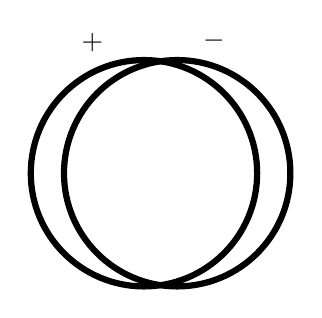
\begin{tikzpicture}[x=0.75pt,y=0.75pt,yscale=-1,xscale=1]
            %uncomment if require: \path (0,300); %set diagram left start at 0, and has height of 300

            %Shape: Circle [id:dp0355540611559928] 
            \draw  [line width=2.25]  (125.23,130.86) .. controls (125.23,100.75) and (149.64,76.33) .. (179.76,76.33) .. controls (209.87,76.33) and (234.29,100.75) .. (234.29,130.86) .. controls (234.29,160.97) and (209.87,185.39) .. (179.76,185.39) .. controls (149.64,185.39) and (125.23,160.97) .. (125.23,130.86) -- cycle ;
            %Shape: Circle [id:dp1469825906597222] 
            \draw  [line width=2.25]  (141.23,130.86) .. controls (141.23,100.75) and (165.64,76.33) .. (195.76,76.33) .. controls (225.87,76.33) and (250.29,100.75) .. (250.29,130.86) .. controls (250.29,160.97) and (225.87,185.39) .. (195.76,185.39) .. controls (165.64,185.39) and (141.23,160.97) .. (141.23,130.86) -- cycle ;

            % Text Node
            \draw (148.5,62) node [anchor=north west][inner sep=0.75pt]   [align=left] {$\displaystyle +$};
            % Text Node
            \draw (207,61) node [anchor=north west][inner sep=0.75pt]   [align=left] {$\displaystyle -$};


        \end{tikzpicture}

        \caption{题图}
    \end{figure}

    球内部使用Gauss定理:

    \begin{align}
        \mathbf{E} \cdot 4\pi r^2 & = \frac{\rho}{\varepsilon_0} \cdot \frac{4}{3}\pi r^3 \hat{\mathbf{r}} \\
        \mathbf{E}                & = \frac{\rho}{3\varepsilon_0} \mathbf{r}
    \end{align}

    从而内部一点的电场:

    \begin{align}
        \mathbf{E} & = \frac{\rho}{3\varepsilon_0} (\mathbf{r}_2-\mathbf{r}_1) \\
                   & = - \frac{\rho}{3\varepsilon_0} \mathbf{P}
    \end{align}


\end{example}

\subsection{电介质中场的方程}

我们对静电场的方程做一个修正:

\begin{align}
    \nabla \cdot \mathbf{E}                              & = \frac{\rho}{\varepsilon_0} = \frac{\rho_0+\rho'}{\varepsilon_0} = \frac{\rho_0-\nabla \cdot \mathbf{P}}{\varepsilon_0} \\
    \nabla \cdot (\varepsilon_0 \mathbf{E} + \mathbf{P}) & = \rho_0
\end{align}

我们定义电位移矢量:

\begin{align}
    \mathbf{D} & = \varepsilon_0 \mathbf{E} + \mathbf{P}
\end{align}

则有:

\begin{align}
    \nabla \cdot \mathbf{D} & = \rho_0
\end{align}

这是电介质中的Gauss定理,其中$\rho_0$是自由电荷密度,$\rho$是总电荷密度。

现在Maxwell方程组变为:

\begin{align}
    \nabla \cdot \mathbf{D}  & = \rho_0 \\
    \nabla \times \mathbf{E} & = 0
\end{align}

对各向同性介质:

\begin{align}
    \mathbf{P} & = \chi_e \varepsilon_0 \mathbf{E}                                                                       \\
    \mathbf{D} & = \varepsilon_0 (1+\chi_e) \mathbf{E} = \varepsilon_0 \varepsilon_r \mathbf{E} = \varepsilon \mathbf{E}
\end{align}

其中$\varepsilon_r$是相对介电常数,$\varepsilon$是介电常数,$\chi_e$是电极化率。

故对于各向同性介质:

\begin{align}
    \nabla \cdot \mathbf{E}  & = \frac{\rho_0}{\varepsilon} = \frac{\rho}{\varepsilon_0} \\
    \nabla \times \mathbf{E} & = 0
\end{align}

\subsection{电介质中的边值关系}

无自由面电荷,在电介质表面取Gauss面,有:

\begin{align}
    \mathbf{D_1} \cdot \mathrm{d} \mathbf{S} - \mathbf{D_2} \cdot \mathrm{d} \mathbf{S} & = Q_0 = 0         \\
    \mathbf{D}_{1n}                                                                     & = \mathbf{D}_{2n}
\end{align}

在电介质表面取回路,有:

\begin{align}
    \mathbf{E_1} \cdot \mathrm{d} \mathbf{l} - \mathbf{E_2} \cdot \mathrm{d} \mathbf{l} & = 0               \\
    \mathbf{E}_{1t}                                                                     & = \mathbf{E}_{2t}
\end{align}

沿着法线方向$\mathbf{D}$连续,沿着切线方向$\mathbf{E}$连续。

也可以写成电势形式:

\begin{align}
    \phi_1 - \phi_2                                                                                   & = 0 \\
    \varepsilon_1\frac{\partial \phi_1}{\partial n} - \varepsilon_2\frac{\partial \phi_2}{\partial n} & = 0
\end{align}

\begin{example}
    对于带电物体外面的两种电介质的边界沿着原来的等势面,或者沿着原来的电场线,都可以用唯一性定理和边界条件,得到和原来形状相同的等势面和电场线。
\end{example}

\chapter{静电能}

\begin{block}{静电能}
    \begin{align}
        W_\text{互} & = \sum_{i\neq j} \frac{1}{8\pi\varepsilon_0} \frac{q_i q_j}{|\mathbf{r}_i-\mathbf{r}_j|} \\
                   & = \frac{1}{2} \int \rho \phi \mathrm{d} V = \frac{1}{2} QU                               \\
                   & = \frac{1}{2} \int \mathbf{E} \cdot \mathbf{D} \mathrm{d} V
    \end{align}

    总静电能=自由电荷系能=总电荷$-$极化电荷系能=宏观电场能+微观电场能:
    \begin{align}
        W & = \frac{1}{2} \int \rho_0 \phi \mathrm{d} V                                                                                         \\
        W & = \frac{1}{2} \int (\rho - \rho')\phi \mathrm{d} V                                                                                  \\
          & = \frac{1}{2} \varepsilon \int \mathbf{E} \cdot \mathbf{E} \mathrm{d} V                                                             \\
          & = \frac{1}{2} \int \mathbf{D} \cdot \mathbf{E} \mathrm{d} V                                                                         \\
          & = \frac{1}{2} \varepsilon \int \mathbf{E} \cdot \mathbf{E} \mathrm{d} V + \frac{1}{2} \int \mathbf{P} \cdot \mathbf{E} \mathrm{d} V
    \end{align}
    静电力:
    \begin{align}
        \mathbf{F} & = \nabla W |_\text{$U$不变}   \\
                   & = - \nabla W |_\text{$Q$不变}
    \end{align}
\end{block}

\newpage

能量是一个标量,利用虚功可以计算力:克服体系中的内力做的功等于体系能量的增加。

\section{点电荷系的静电能}

下面我们计算点电荷系的静电互能:

n个点电荷,先把$q_1,q_2,\cdots,q_n$依次移走,有:
\begin{align}
    W & = q_1 \phi(2,\cdots,n) + q_2 \phi(3,\cdots,n) + \cdots + q_{n-1} \phi(n)
\end{align}

再把$q_1,q_2,\cdots,q_n$依次移回,有:
\begin{align}
    W & = q_1 \phi(1) + q_2 \phi(1,2) + \cdots + q_{n-1} \phi(1,2,\cdots,n-2) + q_n \phi(1,2,\cdots,n-1)
\end{align}

两式相加(即对电势能算两次),得到:
\begin{align}
    W_\text{互} & = \frac{1}{2} \sum q_i \phi(j=1,\cdots,n;j\neq i)                                        \\
               & = \sum_{i\neq j} \frac{1}{8\pi\varepsilon_0} \frac{q_i q_j}{|\mathbf{r}_i-\mathbf{r}_j|} \\
               & = \frac{1}{2}\sum q_i \phi_i
\end{align}

\section{连续电荷分布的静电能}

\begin{align}
    W & = \frac{1}{2} \int \rho \phi \mathrm{d} V        \\
      & =  \frac{1}{2} \int \sigma \phi \mathrm{d} S     \\
      & \neq  \frac{1}{2} \int \lambda \phi \mathrm{d} l
\end{align}

\subsection{体电荷}

计算一个均匀带电球的静电能:
\begin{align}
    W & = \int \phi \mathrm{d} q                                                                   \\
      & = \int_0^R \frac{\rho \frac{4}{3} \pi r^3}{4\pi\varepsilon_0 } \rho 4 \pi r^2 \mathrm{d} r \\
      & = \frac{4\pi\rho^2 R^5}{15\varepsilon_0}
\end{align}

\begin{note}
    \begin{enumerate}
        \item 当$\rho$固定时,$R \rightarrow 0$,$W \rightarrow 0$。这说明无限小体积元 $\rho \mathrm{d} V$ 的静电自能等于零。所以在公式中的$\phi$是可以为所有电荷产生的电势的(不必除去体积微元)。
        \item 当$Q$固定时,$R \rightarrow 0$,$W \rightarrow \infty$。对应点电荷模型,其静电自能发散。(电子自能发散)
        \item 根据公式也可以计算出静电能:
              \begin{align}
                  W & = \frac{1}{2} \int \rho \phi \mathrm{d} V                                    \\
                    & = \frac{1}{2} \int  \frac{\rho^2}{6\pi\varepsilon_0} (3R^2-r^2) \mathrm{d} V \\
                    & = \frac{4\pi\rho^2 R^5}{15\varepsilon_0}
              \end{align}
    \end{enumerate}
\end{note}

\subsection{面电荷}

计算一个均匀带电圆盘的静电能:

考虑其轴线上一点的电势:

\begin{align}
    \phi(z) & = \int \frac{\sigma r \mathrm{d} r \mathrm{d} \theta}{4\pi\varepsilon_0 \sqrt{r^2+z^2}} \\
            & = \frac{\sigma}{2\varepsilon_0} (\sqrt{r^2+z^2} - |z|)
\end{align}

\begin{note}
    \begin{enumerate}
        \item 当$z\rightarrow 0$时,$U = \frac{\sigma R}{2 \varepsilon_0}$。
        \item 当$\sigma$固定时,$z \rightarrow 0$,$\phi \rightarrow 0$。这说明无限小面积元 $\sigma \mathrm{d} S$ 的静电自能为0。所以在公式中的$\phi$是可以为所有电荷产生的电势的(不必除去面积微元)。
    \end{enumerate}
\end{note}

\subsection{线电荷}

计算一个均匀带电线长度为$2L$的静电能:

考虑垂直导线中垂线上一点的电势:

\begin{align}
    \phi(z) & = \int \frac{\lambda \mathrm{d} l}{4\pi\varepsilon_0 \sqrt{L^2+z^2}} \\
            & = \frac{\lambda}{2\pi\varepsilon_0} \ln \frac{\sqrt{L^2+z^2} + L}{r}
\end{align}

当$z \rightarrow 0$时,$U  \rightarrow \infty$。不包含自身贡献时,静电能已经发散,自身贡献也发散。不能够正确定义线电荷的静电能。

\section{两种等价的观点}

真空(或者是把电介质看成真空+极化电荷)中有下面的结论:

能量储存在电荷系中:
\begin{align}
    W & = \frac{1}{2} \sum Q_iU_i
\end{align}

能量储存在电场中:
\begin{align}
    W & = \frac{1}{2} \int \mathbf{E} \cdot  \mathbf{D}\mathrm{d} V = \frac{1}{2} \varepsilon_0 \int \mathbf{E} \cdot  \mathbf{E}\mathrm{d} V
\end{align}

\begin{align}
    W & = \frac{1}{2} \int \rho \phi \mathrm{d} V                                                                                                    \\
      & = \frac{1}{2} \int - \varepsilon_0 \phi \nabla^2 \phi \mathrm{d} V                                                                           \\
      & = \frac{1}{2} \varepsilon_0 \oint \phi \nabla \phi \cdot \mathrm{d} \mathbf{S} + \frac{1}{2} \varepsilon_0 \int |\nabla \phi|^2 \mathrm{d} V \\
      & = \frac{1}{2} \varepsilon_0 \int \mathbf{E} \cdot \mathbf{E} \mathrm{d} V
\end{align}
上面用到了Possion方程。并且对于有界的区域,无穷远处的$\phi \sim \frac{1}{r}$,$\nabla \phi \sim \frac{1}{r^2}$,$S \sim r^2$,从而第一个积分为0。

这意味着电荷系中总电荷能量等于宏观电场能量。

如果加上电介质,有总能:
\begin{align}
    W & = \frac{1}{2} \int \rho_0 \phi \mathrm{d} V                                                                                         \\
      & = \frac{1}{2} \varepsilon \int \mathbf{E} \cdot \mathbf{E} \mathrm{d} V                                                             \\
      & = \frac{1}{2} \int \mathbf{D} \cdot \mathbf{E} \mathrm{d} V                                                                         \\
      & = \frac{1}{2} \varepsilon \int \mathbf{E} \cdot \mathbf{E} \mathrm{d} V + \frac{1}{2} \int \mathbf{P} \cdot \mathbf{E} \mathrm{d} V
\end{align}
对于有电介质的静电场,总静电能是自由电荷(总电荷-极化电荷)的能量,同样也是静电场的能量(自由电荷的能量,宏观电场能)+极化能(极化电荷(偶极子)的能量,微观电场能)。

\subsection{自能与互能}

\begin{align}
    W & = \frac{1}{2} \sum Q_iU_i + \frac{1}{2} \sum Q_iU_j                                                   \\
    W & = \frac{1}{2} \sum \mathbf{E}_i \cdot \mathbf{D}_i + \frac{1}{2} \sum \mathbf{E}_i \cdot \mathbf{D}_j
\end{align}

\begin{example}
    考虑一个平行板电容器,极板间填充介电常数为$\epsilon$的电介质。

    当外接电源给其充电时,电源做的功为:
    \begin{align}
        W & = \int_0^Q U \mathrm{d} Q = \frac{1}{2} \frac{Q^2}{C} = \frac{1}{2} Q U
    \end{align}

    当电容器充满电荷后,电容器的能量为:
    \begin{align}
        W & = \frac{1}{2} Q U = \frac{1}{2} Q^2 \frac{1}{C} = \frac{1}{2} Q^2 \frac{\varepsilon S}{d}
    \end{align}

    而
    \begin{align}
        Q & = P S \\
        U & = E d
    \end{align}

    则:
    \begin{align}
        W & = \frac{1}{2} ED V
    \end{align}

\end{example}

\section{静电能到静电力}

利用虚功求力本质上是能量守恒定律:

克服体系中的内力做的功等于体系能量的增加。
\begin{align}
    - \nabla W & = \mathbf{F}
\end{align}

如果还有其他能量输入,对体系做功$\delta A$,则表达式为:
\begin{align}
    \delta A - \nabla W & = \mathbf{F} \cdot \mathrm{d} \mathbf{l}
\end{align}

\begin{example}
    两个带电导体之间的力(电容器)。

    $Q$不变,则有:
    \begin{align}
        F & =- \frac{\partial W}{\partial x}                            \\
          & = - \frac{1}{2} \frac{\partial Q^2}{\partial x} \frac{1}{C} \\
          & = -\frac{Q^2}{2 \varepsilon S}
    \end{align}

    若按照$U$不变计算,则有电源做功$\delta A = U \mathrm{d} Q$。

\end{example}

详细地:
\begin{align}
    \mathbf{F} & = \nabla W |_\text{$U$不变}   \\
               & = - \nabla W |_\text{$Q$不变}
\end{align}

\chapter{稳恒电流}

\begin{block}{方程}
    \begin{align}
        \quad
        \text{基本方程} \quad & \left\{
        \begin{aligned}
            \nabla \cdot \mathbf{j}  & = \rho_0            & \text{Gauss定理} \\
            \nabla \times \mathbf{E} & = 0                 & \text{环路定理}    \\
            \mathbf{j}               & = \sigma \mathbf{E} & \text{Ohm定律}   \\
        \end{aligned}
        \right.                     \\
        \text{边值关系} \quad
                          & \left\{
        \begin{aligned}
            \mathbf{j}_{1n}                                   & = \mathbf{j}_{2n}                                   \\
            \mathbf{E}_{1t}                                   & = \mathbf{E}_{2t}                                   \\
            \phi_1                                            & =   \phi_2                                          \\
            \varepsilon_1\frac{\partial \sigma_1}{\partial n} & = \varepsilon_2\frac{\partial \sigma_2}{\partial n}
        \end{aligned}
        \right.
    \end{align}
\end{block}

\begin{block}{Kirchhoff定律}
    \begin{align}
        \sum I_i         & = 0           \\
        \sum \mathcal{E} & = \sum I_iR_i
    \end{align}

\end{block}

\newpage

\textbf{电流:}自由电荷宏观定向运动形成电流。

导体脱离静电平衡状态,导体不再是等势体,导体内部有电场。

\textbf{稳恒电流:}电流分布不随时间变化,此时对应电场分布为一稳恒电场。

\section{电流连续性方程与稳恒条件}

\subsection{电流强度、电流密度、电荷密度}

电流密度矢量:
\begin{align}
    \mathbf{j} & = j \hat{\mathbf{n}}                 \\
               & = \rho \mathbf{v}                    \\
    j          & = \frac{\Delta Q}{\Delta t \Delta S}
\end{align}


电流强度:
\begin{align}
    I & = \frac{\mathrm{d} Q}{\mathrm{d} t}           \\
      & = \int \mathbf{j} \cdot \mathrm{d} \mathbf{S}
\end{align}
是一个通量。

面电流密度:
\begin{align}
    \mathbf{i} & = \sigma \mathbf{u}                 \\
    i          & = \frac{\Delta Q}{\Delta t\Delta l} \\
               & = n I
\end{align}

\subsection{电流连续性方程}

电荷守恒方程:
\begin{align}
    \frac{\partial \rho}{\partial t} + \nabla \cdot \mathbf{j} & = 0
\end{align}

稳恒意味着:空间电荷分布不再改变,即$\frac{\partial \rho}{\partial t} = 0$,从而有:

\begin{align}
    \nabla \cdot \mathbf{j} & = 0
\end{align}

物理意义是:电流场线闭合且同一电流管内各截面上$\mathbf{j}$的通量$I$相同。

\subsection{产生稳恒电流}

电源:电容器+用非静电力搬运电荷的小妖。

电源电动势:
\begin{align}
    \mathcal{E} & = \int \mathbf{E}_k \cdot \mathrm{d} \mathbf{l}
\end{align}

非静电力做功:
\begin{align}
    W_k & = \int \mathbf{F}_k \cdot \mathrm{d} \mathbf{l} = \int \mathcal{E} \mathrm{d} Q
\end{align}


\section{稳恒电流与电场}

根据稳恒条件可以得到:
\begin{align}
    \nabla \cdot \mathbf{j}  & = 0 \\
    \nabla \times \mathbf{E} & = 0
\end{align}

\subsection{Ohm定律}

还差一个方程,可以用Ohm定律得到:
\begin{align}
    \mathbf{j} & = \sigma \mathbf{E}
\end{align}
其中$\sigma$是电导率。

\begin{note}
    补齐方程后就有相同的边值条件和唯一性定理。
\end{note}

\begin{align}
    \frac{U}{I} & = \frac{El}{jS}                \\
                & = \frac{1}{\sigma} \frac{L}{S}
\end{align}

\begin{note}
    电阻的经典电子论

    自由电子受电场加速获得速度,然后与晶格碰撞向各个方向散射,宏观平均速度变为零。

    电子从加速后的平均速度表达式为:
    \begin{align}
        \bar{u}_1 = \vec{a} \cdot \tau = -\frac{e\tau \vec{E}}{m}
    \end{align}

    其中平均功率散失在之间平均时间 \(\tau = \frac{\lambda}{\vec{v}}\),而\(\lambda\)为平均自由路径,\(\vec{v}\)为平均热速度。

    电子漂移速度表达式为:
    \begin{align}
        \bar{u} & = \frac{1}{2}(\bar{u}_0 + \bar{u}_1)        \\
                & = -\frac{e\bar{\lambda} \vec{E}}{2m\bar{v}}
    \end{align}

    电流密度:
    \begin{align}
        \vec{j} & = -ne\bar{u} = -\frac{ne^2\bar{\lambda}}{2m\bar{v}}\vec{E}
    \end{align}

    从而电导率:
    \begin{align}
        \sigma & = \frac{j}{E} = \frac{ne^2\bar{\lambda}}{2m\bar{v}}
    \end{align}
    其中 \(\vec{v} \propto \sqrt{T}\),因此 \(\rho \propto \frac{\vec{v}}{n\lambda}\), 从而电阻率 \(\rho \propto \sqrt{T}\)。

\end{note}

\subsection{Joule定律}

\begin{align}
    P & = U I = \frac{U^2}{R} = I^2 R \\
      & = \frac{j^2}{\sigma}
\end{align}

\subsection{稳恒电流的方程}

\begin{align}
    \quad
     & \left\{
    \begin{aligned}
        \nabla \cdot \mathbf{j}  & = \rho_0            & \text{Gauss定理} \\
        \nabla \times \mathbf{E} & = 0                 & \text{环路定理}    \\
        \mathbf{j}               & = \sigma \mathbf{E} & \text{Ohm定律}   \\
    \end{aligned}
    \right.    \\
    \text{边值关系} \quad
     & \left\{
    \begin{aligned}
        \mathbf{j}_{1n}                                   & = \mathbf{j}_{2n}                                   \\
        \mathbf{E}_{1t}                                   & = \mathbf{E}_{2t}                                   \\
        \phi_1                                            & =   \phi_2                                          \\
        \varepsilon_1\frac{\partial \sigma_1}{\partial n} & = \varepsilon_2\frac{\partial \sigma_2}{\partial n}
    \end{aligned}
    \right.
\end{align}

\subsection{导体内部和表面电场}

\begin{figure}[ht]
    \centering


    \tikzset{every picture/.style={line width=0.75pt}} %set default line width to 0.75pt        

    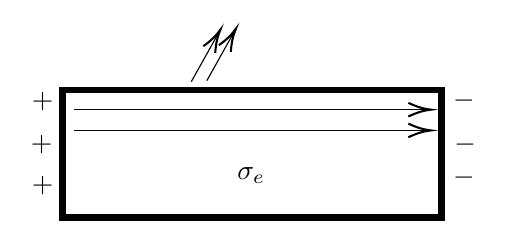
\begin{tikzpicture}[x=0.75pt,y=0.75pt,yscale=-1,xscale=1]
        %uncomment if require: \path (0,300); %set diagram left start at 0, and has height of 300

        %Shape: Rectangle [id:dp5785582177969313] 
        \draw  [line width=2.25]  (50,60) -- (232.57,60) -- (232.57,121.55) -- (50,121.55) -- cycle ;
        %Straight Lines [id:da9748245052671594] 
        \draw    (55.57,69.55) -- (225.57,69.55) ;
        \draw [shift={(227.57,69.55)}, rotate = 180] [color={rgb, 255:red, 0; green, 0; blue, 0 }  ][line width=0.75]    (10.93,-3.29) .. controls (6.95,-1.4) and (3.31,-0.3) .. (0,0) .. controls (3.31,0.3) and (6.95,1.4) .. (10.93,3.29)   ;
        %Straight Lines [id:da9634404771274951] 
        \draw    (55.57,79.55) -- (225.57,79.55) ;
        \draw [shift={(227.57,79.55)}, rotate = 180] [color={rgb, 255:red, 0; green, 0; blue, 0 }  ][line width=0.75]    (10.93,-3.29) .. controls (6.95,-1.4) and (3.31,-0.3) .. (0,0) .. controls (3.31,0.3) and (6.95,1.4) .. (10.93,3.29)   ;
        %Straight Lines [id:da48861161237822226] 
        \draw    (112.07,56.05) -- (125.09,32.8) ;
        \draw [shift={(126.07,31.05)}, rotate = 119.25] [color={rgb, 255:red, 0; green, 0; blue, 0 }  ][line width=0.75]    (10.93,-3.29) .. controls (6.95,-1.4) and (3.31,-0.3) .. (0,0) .. controls (3.31,0.3) and (6.95,1.4) .. (10.93,3.29)   ;
        %Straight Lines [id:da6076677557069543] 
        \draw    (119.57,55.55) -- (132.59,32.3) ;
        \draw [shift={(133.57,30.55)}, rotate = 119.25] [color={rgb, 255:red, 0; green, 0; blue, 0 }  ][line width=0.75]    (10.93,-3.29) .. controls (6.95,-1.4) and (3.31,-0.3) .. (0,0) .. controls (3.31,0.3) and (6.95,1.4) .. (10.93,3.29)   ;

        % Text Node
        \draw (34,60) node [anchor=north west][inner sep=0.75pt]   [align=left] {$\displaystyle +$};
        % Text Node
        \draw (33.5,80.5) node [anchor=north west][inner sep=0.75pt]   [align=left] {$\displaystyle +$};
        % Text Node
        \draw (34,100.5) node [anchor=north west][inner sep=0.75pt]   [align=left] {$\displaystyle +$};
        % Text Node
        \draw (237,59.5) node [anchor=north west][inner sep=0.75pt]   [align=left] {$\displaystyle -$};
        % Text Node
        \draw (237.5,80.5) node [anchor=north west][inner sep=0.75pt]   [align=left] {$\displaystyle -$};
        % Text Node
        \draw (237,96.5) node [anchor=north west][inner sep=0.75pt]   [align=left] {$\displaystyle -$};
        % Text Node
        \draw (133,96) node [anchor=north west][inner sep=0.75pt]   [align=left] {$\displaystyle \sigma _{e}$};


    \end{tikzpicture}
    \caption{导体内部和表面电场}
\end{figure}

\begin{align}
    \mathbf{j}_\text{n外} & = 0                                                  \\
    \mathbf{j}_\text{n内} & = 0                                                  \\
    \mathbf{E}_\text{n内} & = 0                                                  \\
    \mathbf{E}_\text{t外} & = \mathbf{E}_\text{t内} = \frac{\mathbf{j}}{\sigma_e} \\
    \mathbf{E}_\text{n外} & = \frac{\sigma}{\varepsilon_0}
\end{align}

导体表面是有电荷的,这样才能约束内部电场线平行于导体表面。

\section{Kirchhoff定律}

\subsection{电流定律}

\begin{align}
    \sum I_\text{in} & = \sum I_\text{out}
\end{align}

\begin{proof}
    利用第一个方程的Gauss定律:
    \begin{align}
        \int \mathbf{j}_\text{in} \cdot \mathrm{d} \mathbf{S}  =0
    \end{align}

    \begin{align}
        \sum I_\text{in} & = \sum \int \mathbf{j}_\text{in} \cdot \mathrm{d} \mathbf{S}  \\
                         & = \sum \int \mathbf{j}_\text{out} \cdot \mathrm{d} \mathbf{S} \\
                         & = \sum I_\text{out}
    \end{align}
\end{proof}

\subsection{电动势定律}

\begin{align}
    \sum \mathcal{E} & = \sum I_iR_i
\end{align}

\begin{proof}
    利用第二个方程的环路定理:
    \begin{align}
        \oint \mathbf{E} \cdot \mathrm{d} \mathbf{l}  =0
    \end{align}

    且电流密度有:
    \begin{align}
        \mathbf{j} & = \sigma (\mathbf{E}+\mathbf{E}_k)
    \end{align}

    \begin{align}
        \sum \mathcal{E} & = \oint \mathbf{E}_k \cdot \mathrm{d} \mathbf{l}                                                                 \\
                         & = \oint \frac{\mathbf{j}}{\sigma} \cdot \mathrm{d} \mathbf{l}                                                    \\
                         & = \oint \frac{\mathbf{j} \mathrm{d} \mathbf{S} \cdot \mathrm{d} \mathbf{l} }{\sigma \cdot \mathrm{d} \mathbf{S}} \\
                         & = \sum I_iR_i
    \end{align}
\end{proof}

\chapter{真空中的静磁场}

\begin{block}{方程}
    \begin{align}
        \quad
        \text{基本方程} \quad & \left\{
        \begin{aligned}
            \nabla \cdot \mathbf{B}  & = 0                \\
            \nabla \times \mathbf{B} & = \mu_0 \mathbf{j} \\
        \end{aligned}
        \right.                     \\
        \text{积分形式} \quad
                          & \left\{
        \begin{aligned}
            \oint \mathbf{B} \cdot \mathrm{d} \mathbf{S} & = 0       \\
            \oint \mathbf{B} \cdot \mathrm{d} \mathbf{l} & = \mu_0 I
        \end{aligned}
        \right.
    \end{align}
\end{block}

\begin{block}{磁矢量势}
    \begin{align}
        \nabla \cdot \mathbf{A}                      & = 0                                           \\
        \nabla \times \mathbf{A}                     & = \mathbf{B}                                  \\
        \oint \mathbf{A} \cdot \mathrm{d} \mathbf{l} & = \int \mathbf{B} \cdot \mathrm{d} \mathbf{S}
    \end{align}
\end{block}

\begin{block}{螺线管}
    \begin{align}
        \mathbf{B}_0         & = \frac{\mu_0 n I}{2} (\frac{z_2}{\sqrt{r^2+z_2^2}}-\frac{z_1}{\sqrt{r^2+z_1^2}})\hat{\mathbf{z}} \\
        \mathbf{B}_\text{t内} & = \mu_0 n I                                                                                       \\
        \mathbf{B}_\text{t外} & = 0                                                                                               \\
        \mathbf{B}_\text{n内} & = 0                                                                                               \\
        \mathbf{B}_\text{n外} & = \mu_0 I
    \end{align}
\end{block}

\begin{block}{Lorentz力}
    \begin{align}
        \mathbf{F} & = q(\mathbf{E} + \mathbf{v} \times \mathbf{B})
    \end{align}
\end{block}


\begin{block}{常数}
    \begin{align}
        \mu_0 & = 4\pi \times 10^{-7} \mathrm{N/A^2}
    \end{align}
\end{block}

\newpage

\section{Oersted实验}

电流的磁效应

\section{Biot-Savart-Laplace定律}

电流元产生的磁场:
\begin{align}
    \mathrm{d} \mathbf{B} & = \frac{\mu_0}{4\pi} \frac{I \mathrm{d} \mathbf{l} \times \mathbf{r}}{r^3}    \\
                          & = \frac{\mu_0}{4\pi}  \frac{  \mathbf{j} \times \mathbf{r}}{r^3} \mathrm{d} V
\end{align}

从而:
\begin{align}
    \mathbf{B} & = \frac{\mu_0}{4\pi} \int \frac{  \mathbf{j} \times \mathbf{r}}{r^3} \mathrm{d} V \\
               & = \frac{\mu_0}{4\pi} \int \frac{  \mathbf{i} \times \mathbf{r}}{r^3} \mathrm{d} S \\
               & = \frac{\mu_0}{4\pi} \int \frac{I  \mathrm{d}\mathbf{l} \times \mathbf{r}}{r^3}
\end{align}

\subsection{常见磁场举例}

\begin{enumerate}
    \item 有限长直流导线
          \begin{align}
              \mathbf{B} & = \frac{\mu_0 I}{4\pi}(\sin \theta_2 - \sin \theta_1) \hat{\mathbf{y}}
                         & = \frac{\mu_0 I}{4\pi} (\frac{z_2}{\sqrt{z_2^2 + a^2}} - \frac{z_1}{\sqrt{z_1^2 + a^2}}) \hat{\mathbf{y}}
          \end{align}
    \item 电流环轴线
          \begin{align}
              \mathbf{B} & = \frac{\mu_0 I}{2} \frac{r^2}{(r^2+z^2)^\frac{3}{2}}\hat{\mathbf{z}}
          \end{align}
    \item 有限长螺线管

          相当于多个电流环叠加,有:
          \begin{align}
              \mathbf{B} & = \frac{\mu_0 n I}{2} (\frac{z_2}{\sqrt{r^2+z_2^2}}-\frac{z_1}{\sqrt{r^2+z_1^2}})\hat{\mathbf{z}}
          \end{align}
          其中$n$为单位长度的匝数。
\end{enumerate}

\section{Ampere定律}

两个电流元之间的相互作用力沿他们的连线:

\begin{align}
    \mathrm{d} \mathbf{F} & = -\frac{\mu_0}{4\pi} \frac{I_1 I_2 \mathrm{d} \mathbf{l}_1 \times (\mathrm{d} \mathbf{l}_2 \times \mathbf{r})}{r^3}
\end{align}

\section{静磁场的基本定理}

\subsection{静磁场的基本方程}

从Biot-Savart-Laplace定律和叠加原理出发,可以得到静磁场的基本方程:
\begin{align}
    \nabla \cdot \mathbf{B}  & = \nabla \cdot \int \frac{\mu_0}{4\pi} \frac{  \mathbf{j} \times \mathbf{r}}{r^3} \mathrm{d} V   \\
                             & = \int \frac{\mu_0}{4\pi} \nabla \cdot \frac{  \mathbf{j} \times \mathbf{r}}{r^3} \mathrm{d} V   \\
                             & = \int \frac{\mu_0}{4\pi} \mathbf{j} \cdot  \nabla  \times(\frac{ \mathbf{r}}{r^3}) \mathrm{d} V \\
                             & = 0                                                                                              \\
    \nabla \times \mathbf{B} & = \nabla \times \int \frac{\mu_0}{4\pi} \frac{  \mathbf{j} \times \mathbf{r}}{r^3} \mathrm{d} V  \\
                             & = \int \frac{\mu_0}{4\pi} \nabla \times \frac{  \mathbf{j} \times \mathbf{r}}{r^3} \mathrm{d} V  \\
                             & = \cdots                                                                                         \\
                             & = \mu_0 \mathbf{j}
\end{align}

\subsection{方程的积分形式}
他们的积分形式为:
\begin{align}
    \oint \mathbf{B} \cdot \mathrm{d} \mathbf{S} & = 0       \\
    \oint \mathbf{B} \cdot \mathrm{d} \mathbf{l} & = \mu_0 I
\end{align}

\subsection{磁矢量势}

如同静电场可以定义电势,静磁场也可以定义磁矢量势$\mathbf{A}$,满足:
\begin{align}
    \mathbf{B} & = \nabla \times \mathbf{A}
\end{align}

如同电势一样,我们可以写出磁矢量势的Poisson方程:
\begin{align}
    \nabla^2 \mathbf{A} & = -\mu_0 \mathbf{j}
\end{align}

\begin{note}
    磁矢量势不唯一。
\end{note}

我们遵循Coloumb规范:
\begin{align}
    \nabla \cdot \mathbf{A} & = 0
\end{align}

\begin{align}
    \nabla \cdot \mathbf{A}  & = 0          \\
    \nabla \times \mathbf{A} & = \mathbf{B}
\end{align}
这两个式子给出了磁矢量势的唯一性。磁矢量势的表达式可以写成:
\begin{align}
    \mathbf{A} & = \frac{\mu_0}{4\pi} \int \frac{  \mathbf{j} (\mathbf{r})}{r} \mathrm{d} V
\end{align}
是一个极矢量。


可以得到其积分形式:
\begin{align}
    \oint \mathbf{A} \cdot \mathrm{d} \mathbf{l} & = \int \mathbf{B} \cdot \mathrm{d} \mathbf{S}
\end{align}
我们通常利用这个式子来计算磁矢量势。

\begin{example}
    无限长螺线管的矢量势。

    \begin{align}
        \int \mathbf{B} \cdot \mathrm{d} \mathbf{S} & = \oint \mathbf{A} \cdot \mathrm{d} \mathbf{l}
    \end{align}

    从而:
    \begin{align}
        A & = \frac{BS_0}{2\pi r}
    \end{align}
\end{example}

\section{对称性原理及应用}

\subsection{对称与反对称的定义}

一个物理场经过某种对称操作S后,形成新物理场
\begin{itemize}
    \item 对称:变换后的场与变换前的场完全相同,则称该场具有对称性。
    \item 反对称:变换后的场与变换前的场相差一个负号,则称该场具有反对称性。
\end{itemize}

\subsection{极矢量与轴矢量}

\begin{itemize}
    \item 极矢量:可以通过$\mathbf{r}$表示的,例如:$\mathbf{r},\mathbf{v}= \frac{\mathrm{d} \mathbf{r}}{\mathrm{d} t},\mathbf{p}=m\mathbf{v},\mathbf{j}=\rho \mathbf{v}$等。
    \item 轴矢量:两个极矢量的叉积,例如:$\mathbf{L}=\mathbf{r} \times \mathbf{p},\mathbf{M}=\mathbf{r} \times \mathbf{F}$等。
\end{itemize}

\subsection{对称性法则}

源的对称性带来场的对称性。

源具有标量的对称性,则场具有极矢量、轴矢量的对称性。

例如对于y-z平面对称:
\begin{align}
    E_{\parallel}(-x,y,z) & = E_{\parallel}(x,y,z) \\
    E_{\perp}(-x,y,z)     & = -E_{\perp}(x,y,z)
\end{align}
\begin{align}
    B_{\parallel}(-x,y,z) & = - B_{\parallel}(x,y,z) \\
    B_{\perp}(-x,y,z)     & = B_{\perp}(x,y,z)
\end{align}

而关于y-z平面反对称:
\begin{align}
    E_{\parallel}(-x,y,z) & = -E_{\parallel}(x,y,z) \\
    E_{\perp}(-x,y,z)     & = E_{\perp}(x,y,z)
\end{align}
\begin{align}
    B_{\parallel}(-x,y,z) & = B_{\parallel}(x,y,z) \\
    B_{\perp}(-x,y,z)     & = -B_{\perp}(x,y,z)
\end{align}

\subsection{对称性法则的应用}

如下面三个图:

\begin{figure}[ht]
    \centering
    \includegraphics[width=0.6\textwidth]{pic/6.5.4.3.png}
    \caption{对称性法则的应用}
\end{figure}

\begin{figure}[ht]
    \centering
    \includegraphics[width=0.5\textwidth]{pic/6.5.4.1.png}
    \caption{对称性法则的应用}
\end{figure}

\begin{figure}[ht]
    \centering
    \includegraphics[width=0.5\textwidth]{pic/6.5.4.2.png}
    \caption{对称性法则的应用}
\end{figure}

\newpage

\begin{example}
    无限长通电螺线管的磁场。

    \textbf{先计算轴向磁场:}
    用前面的结论,可以得到,轴线上的磁场为:
    \begin{align}
        B_0 & = \mu_0 n I
    \end{align}

    取上图的那两个回路,可以得到:
    \begin{align}
        B_0 \Delta l - B_\text{外} \Delta l & = \mu_0 n I \Delta l \\
        B_0 \Delta l - B_\text{内} \Delta l & = 0
    \end{align}

    从而内部是匀强磁场,外部是无磁场。

    \textbf{再计算垂直于轴的磁场:}

    \begin{figure}[ht]
        \centering


        \tikzset{every picture/.style={line width=0.75pt}} %set default line width to 0.75pt        

        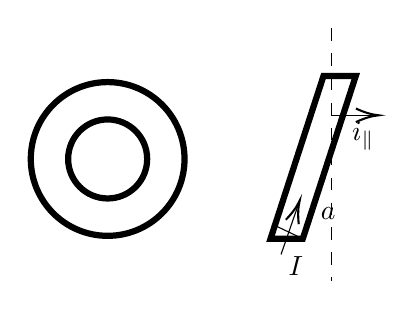
\begin{tikzpicture}[x=0.75pt,y=0.75pt,yscale=-1,xscale=1]
            %uncomment if require: \path (0,300); %set diagram left start at 0, and has height of 300

            %Shape: Circle [id:dp6032105635792695] 
            \draw  [line width=2.25]  (50,96.04) .. controls (50,75.58) and (66.58,59) .. (87.04,59) .. controls (107.49,59) and (124.07,75.58) .. (124.07,96.04) .. controls (124.07,116.49) and (107.49,133.07) .. (87.04,133.07) .. controls (66.58,133.07) and (50,116.49) .. (50,96.04) -- cycle ;
            %Shape: Circle [id:dp9176095898614838] 
            \draw  [line width=2.25]  (68,96.04) .. controls (68,85.52) and (76.52,77) .. (87.04,77) .. controls (97.55,77) and (106.07,85.52) .. (106.07,96.04) .. controls (106.07,106.55) and (97.55,115.07) .. (87.04,115.07) .. controls (76.52,115.07) and (68,106.55) .. (68,96.04) -- cycle ;
            %Shape: Parallelogram [id:dp5085428546048079] 
            \draw  [line width=2.25]  (191.03,56.05) -- (206.57,56.05) -- (181.04,134.5) -- (165.5,134.5) -- cycle ;
            %Straight Lines [id:da25791954464421507] 
            \draw    (181.04,134.5) -- (167.57,128.05) ;
            %Straight Lines [id:da7640739860865882] 
            \draw    (170.57,142.05) -- (178.92,117.94) ;
            \draw [shift={(179.57,116.05)}, rotate = 109.09] [color={rgb, 255:red, 0; green, 0; blue, 0 }  ][line width=0.75]    (10.93,-3.29) .. controls (6.95,-1.4) and (3.31,-0.3) .. (0,0) .. controls (3.31,0.3) and (6.95,1.4) .. (10.93,3.29)   ;
            %Straight Lines [id:da1266946959090074] 
            \draw  [dash pattern={on 4.5pt off 4.5pt}]  (195,33.05) -- (195,155.05) ;
            %Straight Lines [id:da869324026727873] 
            \draw    (194.5,75) -- (215.57,75) ;
            \draw [shift={(217.57,75)}, rotate = 180] [color={rgb, 255:red, 0; green, 0; blue, 0 }  ][line width=0.75]    (10.93,-3.29) .. controls (6.95,-1.4) and (3.31,-0.3) .. (0,0) .. controls (3.31,0.3) and (6.95,1.4) .. (10.93,3.29)   ;

            % Text Node
            \draw (173,142) node [anchor=north west][inner sep=0.75pt]   [align=left] {$\displaystyle I$};
            % Text Node
            \draw (188.5,118) node [anchor=north west][inner sep=0.75pt]   [align=left] {$\displaystyle a$};
            % Text Node
            \draw (203.5,77) node [anchor=north west][inner sep=0.75pt]   [align=left] {$\displaystyle i_{\parallel }$};


        \end{tikzpicture}

        \caption{无限长通电螺线管的磁场}
    \end{figure}

    对于螺线管的横截面,面电流密度:
    \begin{align}
        i = \frac{I}{a}
    \end{align}
    其中$a$为导线的直径。

    从而,平行和垂直截面的电流密度是:
    \begin{align}
        i_{\perp}     & = i \cos \theta = nI \\
        i_{\parallel} & = i \sin \theta
    \end{align}
    $i_{\perp}$乘长度可以得到过轴线平面剖开的一定长度通过的电流,$i_{\perp}$乘$\frac{a}{\sin\theta}$就是垂直轴线剖开的截面通过的电流即$I$。

    取环路:
    \begin{align}
        B_\text{内} 2 \pi r & = \mu_0 i_{\parallel} = 0            \\
        B_\text{外} 2 \pi r & = \mu_0 i_{\perp} = \mu_0 I \Delta l
    \end{align}

    从而内部无磁场,外部垂直方向的磁场为:
    \begin{align}
        B & = \frac{\mu_0 I}{2\pi r}
    \end{align}

\end{example}


\section{带电粒子在磁场中的运动}

\subsection{Lorentz力}

带电粒子在磁场中的运动方程为:
\begin{align}
    \mathbf{F} & = q(\mathbf{v} \times \mathbf{B})
\end{align}

洛仑兹力不做功:
\begin{align}
    \mathrm{d} W & = \mathbf{F} \cdot \mathrm{d} \mathbf{l} = q( \mathbf{v} \times \mathbf{B}) \cdot \mathbf{v} \mathrm{d} t =0
\end{align}

公式中的$\mathbf{v}$是相对观测者的速度。在导线静止的参照系,电荷受到Lorentz力;而在电荷静止的参照系,电荷受到电场力。磁场和电场是在不同参照系下相互转换。

\subsection{Ampere力}

\begin{align}
    \mathrm{d} \mathbf{F} & = I_1 \mathrm{d} \mathbf{l}_1 \times \mathbf{B}_2
\end{align}

\subsection{带电粒子在磁场中的运动}

由Newton第二定律和Lorentz力,可以得到:
\begin{align}
    \frac{\mathrm{d} m\mathbf{v}}{\mathrm{d} t} & = q(\mathbf{v} \times \mathbf{B})
\end{align}

解得:
\begin{align}
    v_x & = v_{0} \cos \omega t                \\
    v_y & = - \frac{q}{|q|}v_{0} \sin \omega t \\
    v_z & = v_{z0}
\end{align}
其中$\omega = \frac{qB}{m}$。

\subsection{回旋磁矩}

\begin{align}
    \mathbf{\mu} & = I \mathbf{S} = \frac{v_0^2}{2B}
\end{align}
其中$\mathbf{S}=\frac{1}{2}\oint \mathbf{r} \times \mathrm{d} \mathbf{r}$。

磁矩在匀强磁场,或者缓慢变化的磁场中,回旋磁矩守恒。

\subsection{Hall效应}

在电流$I$通过的导体上,有磁场$\mathbf{B}$,则会有Hall电场:
\begin{align}
    \mathbf{E}_H & = \frac{1}{nq} \mathbf{j} \times \mathbf{B} \\
    \mathbf{U}_H & = \frac{IB}{nbq}                            \\
    K_H          & = \frac{1}{nq}                              \\
    R_H          & = \frac{U_H}{I} =  \frac{B}{nbq}
\end{align}

利用带电微粒的平衡条件即可:
\begin{align}
    q\mathbf{E} + q(\mathbf{v} \times \mathbf{B}) = 0
\end{align}

\chapter{静磁场中的磁介质}

\begin{block}{方程}
    \begin{align}
        \quad
        \text{基本方程} & \left\{
        \begin{aligned}
            \nabla \cdot \mathbf{B}  & = 0                \\
            \nabla \times \mathbf{H} & = \mathbf{j}       \\
            \mathbf{B}               & = \mu_0 \mathbf{H}
        \end{aligned}
        \right.               \\
        \text{边值关系} \quad
                    & \left\{
        \begin{aligned}
            \mathbf{B}_{1n} & = \mathbf{B}_{2n} \\
            \mathbf{H}_{1t} & = \mathbf{H}_{2t}
        \end{aligned}
        \right.
    \end{align}
\end{block}

\begin{block}{Ampere 力}
    \begin{align}
        \mathrm{d} \mathbf{F} & = I \mathrm{d} \mathbf{l} \times  \mathbf{B}
    \end{align}
\end{block}

\begin{block}{磁介质}
    \begin{align}
                    & \text{磁化磁介质 = 真空 + 磁化面电流$\mathbf{i}'$ + 磁化体电流$\mathbf{j}'$}             \\
        \mathbf{i}' & = \mathbf{M} \times \hat{\mathbf{n}}                                    \\
        \mathbf{j}' & = \nabla \times \mathbf{M}                                              \\
        \mathbf{M}  & = \chi_m \mathbf{H}                                                     \\
        \mathbf{B}  & = \mu_0 (1+\chi_m) \mathbf{H} = \mu_0 \mu_r \mathbf{H} = \mu \mathbf{H}
    \end{align}
\end{block}

\newpage

\section{磁场对电流的作用}

\subsection{Ampere力}

\subsubsection{电流元的Ampere力}

\begin{align}
    \mathrm{d} \mathbf{F} & = \mathrm{d} N q \mathbf{v} \times \mathbf{B}                             \\
                          & =  n q \mathbf{v} \times \mathbf{B} \mathrm{d} V                          \\
                          & = \rho \mathbf{v} \times \mathbf{B} \mathrm{d} V                          \\
                          & = \mathbf{j} \times \mathbf{B} \mathrm{d} V                               \\
                          & = (\mathbf{j} \times \mathbf{B})( \mathbf{S} \cdot \mathrm{d} \mathbf{l}) \\
                          & = (\mathrm{d} \mathbf{l} \times \mathbf{B})  (\mathbf{S}\cdot \mathbf{j}) \\
                          & = \mathrm{d} \mathbf{l} \times \mathbf{B}\cdot I                          \\
                          & = I \mathrm{d} \mathbf{l} \times \mathbf{B}
\end{align}
其中用到了电流密度$\mathbf{j}$和电流$ \mathbf{v}$是平行的。

\subsubsection{面电流元的Ampere力}

\begin{align}
    \mathrm{d} \mathbf{F} & =  \mathbf{i} \times \mathbf{B}\mathrm{d} S
\end{align}

\subsection{Ampere力与力矩}

\begin{align}
    \mathbf{F} & = q\mathbf{v} \times \mathbf{B}                       \\
    \mathbf{F} & = \oint_{L} I \mathrm{d} \mathbf{l} \times \mathbf{B} \\
    \mathbf{F} & = \int_{S} \mathbf{i} \times \mathbf{B} \mathrm{d} S  \\
    \mathbf{F} & = \int_{V} \mathbf{j} \times \mathbf{B} \mathrm{d} V
\end{align}

\begin{align}
    \mathbf{\tau} & = \int \mathbf{r} \times \mathrm{d} \mathbf{F}                            \\
    \mathbf{\tau} & = \oint_{L} \mathbf{r} \times (I \mathrm{d} \mathbf{l} \times \mathbf{B}) \\
    \mathbf{\tau} & = \int_{S} \mathbf{r} \times (\mathbf{i} \times \mathbf{B}) \mathrm{d} S  \\
    \mathbf{\tau} & = \int_{V} \mathbf{r} \times (\mathbf{j} \times \mathbf{B}) \mathrm{d} V
\end{align}

\begin{example}
    两根无限长平行直载流导线,电流强度$I_1I_2$,相距$r$,求其中一根单位长度受的力。

    $I_1$在$I_2$处产生的磁感应强度:
    \begin{align}
        B & = \frac{\mu_0 I_1}{2\pi r}
    \end{align}

    单位长度导线受到的力:
    \begin{align}
        F & = I_2  \times B                \\
          & = \frac{\mu_0 I_1 I_2}{2\pi r}
    \end{align}

\end{example}

\begin{example}
    求电流强度为$I$,单位长度匝数为$n$的无穷长载流螺线管单位表面受的力。

    \textbf{该无穷长载流螺线管可简化为面电流密度$\mathbf{i}=nI$的面电流分布管。}

    总磁感应强度为:
    \begin{align}
        B_\text{t内} & = \mu_0 n I \\
        B_\text{t外} & = 0
    \end{align}

    面元产生的磁感应强度:
    \begin{align}
        B_\text{0内} & = \frac{\mu_0 n I}{2}  \\
        B_\text{0外} & = -\frac{\mu_0 n I}{2}
    \end{align}

    面元所处的外场:
    \begin{align}
        B & = B_T - B_0 =\frac{\mu_0 n I}{2}
    \end{align}

    面元受到的力:
    \begin{align}
        \mathrm{d} \mathbf{F} & = \mathbf{i} \times \mathbf{B} \mathrm{d}S \\
    \end{align}

    从而单位面积受到的力(垂直于面元指向管外)为:
    \begin{align}
        \frac{\mathrm{d} \mathbf{F}}{\mathrm{d} \mathbf{S}} & = \frac{\mu_0 n^2 I^2}{2}
    \end{align}

    \textbf{正如上一章节分析其磁感应强度。进一步考虑轴向电流的作用,等效成面电流密度$\mathbf{i}=\frac{I}{2\pi R}$的面电流分布管。}

    总磁感应强度为:
    \begin{align}
        B_\text{t内} & = \frac{\mu_0 I}{2\pi R} \\
        B_\text{t外} & = 0
    \end{align}

    面元产生的磁感应强度:
    \begin{align}
        B_\text{0内} & = \frac{\mu_0 I}{4\pi R}  \\
        B_\text{0外} & = -\frac{\mu_0 I}{4\pi R}
    \end{align}

    面元所处的外场:
    \begin{align}
        B & = B_T - B_0 =\frac{\mu_0 I}{4\pi R}
    \end{align}

    面元受到的力:
    \begin{align}
        \mathrm{d} \mathbf{F} & = \mathbf{i} \times \mathbf{B} \mathrm{d}S \\
    \end{align}

    从而单位面积受到的力(垂直于面元指向轴线)为:
    \begin{align}
        \frac{\mathrm{d} \mathbf{F}}{\mathrm{d} \mathbf{S}} & = \frac{\mu_0 I^2}{8 \pi^2R^2}
    \end{align}
\end{example}

\begin{example}
    求一电流强度为$I$的载流线圈在均匀磁场中受到的力和力矩。

    受力:
    \begin{align}
        \mathbf{F} & = \oint I \mathrm{d} \mathbf{l} \times \mathbf{B}   \\
                   & = I (\oint \mathrm{d} \mathbf{l}) \times \mathbf{B} \\
                   & = 0
    \end{align}

    受力矩:
    \begin{align}
        \mathbf{\tau} & = \oint I\mathbf{r} \times (\mathrm{d} \mathbf{l} \times \mathbf{B})                                                                                                                                    \\
                      & = \frac{I}{2}(\oint (\mathbf{r} \times \mathrm{d} \mathbf{r})\times \mathbf{B} + \oint \mathrm{d} \mathbf{r} (\mathbf{r}\cdot \mathbf{B}) - 2\oint\mathbf{B} (\mathbf{r} \cdot \mathrm{d} \mathbf{r}) ) \\
                      & = \frac{I}{2}\oint (\mathbf{r} \times \mathrm{d} \mathbf{r})\times \mathbf{B}                                                                                                                           \\
                      & =  \mathbf{m} \times \mathbf{B}
    \end{align}
    其中$\mathbf{m} = \frac{I}{2}\oint \mathbf{r} \times \mathrm{d} \mathbf{r} = I \mathbf{S}$为磁矩。第二个积分是全微分的回路积分,第三个积分$\mathbf{r} \cdot \mathrm{d} \mathbf{r}= \mathrm{d}(\frac{r^2}{2})$,故两项均为0。

\end{example}

\section{磁介质及其磁化强度}

\subsection{磁偶极子}
我们仿照研究电介质时候使用多级展开的方法:
\begin{align}
    \frac{1}{|\mathbf{X}-\mathbf{X}'|} & = \frac{1}{|\mathbf{X}|} + \frac{\hat{\mathbf{X}} \cdot \mathbf{X}'}{|\mathbf{X}|^2} + \frac{3(\hat{\mathbf{X}} \cdot \mathbf{X}')^2 - |\mathbf{X}'|^2}{2|\mathbf{X}|^3} + \cdots
\end{align}

二者展开是一致的:
\begin{align}
     & \phi(\mathbf{X})          = \frac{1}{4\pi\epsilon_0} \int \frac{\rho(\mathbf{X}')\mathrm{d}^3\mathbf{X}'}{|\mathbf{X} - \mathbf{X}'|}         &
     & \mathbf{A}(\mathbf{X})    = \frac{\mu_0}{4\pi} \int \frac{\mathbf{j}(\mathbf{X}')\mathrm{d}^3\mathbf{X}'}{|\mathbf{X} - \mathbf{X}'|}           \\
     & \mathbf{E}(\mathbf{X})    = -\nabla \phi(\mathbf{X})                                                                                          &
     & \mathbf{B}(\mathbf{X})    = \nabla \times \mathbf{A}(\mathbf{X})                                                                                \\
     & \phi_m(\mathbf{X})        = \frac{1}{4\pi\epsilon_0} \int \frac{\rho(\mathbf{X}')\mathrm{d}^3\mathbf{X}'}{|\mathbf{X}|}                       &
     & \mathbf{A}_m(\mathbf{X})  = \frac{\mu_0}{4\pi} \int \frac{\mathbf{j}(\mathbf{X}')\mathrm{d}^3\mathbf{X}'}{|\mathbf{X}|} = 0                     \\
     & \phi_d(\mathbf{X})        = \frac{\mathbf{\hat{x}} \cdot \mathbf{p}}{4\pi\epsilon_0 |\mathbf{X}|^2}                                           &
     & \mathbf{A}_d(\mathbf{X})  = \frac{\mu_0 \mathbf{m} \times \mathbf{\hat{x}}}{4\pi |\mathbf{X}|^2}                                                \\
     & \mathbf{p}                = \int \rho(\mathbf{X}')\mathbf{X}'\mathrm{d}^3\mathbf{X}' = q\mathbf{d}                                            &
     & \mathbf{m}                = \frac{1}{2} \int \mathbf{X}' \times \mathbf{j}(\mathbf{X}')\mathrm{d}^3\mathbf{X}' = I\mathbf{S}                    \\
     & \mathbf{E}_d(\mathbf{X})  = \frac{1}{4\pi\epsilon_0} \frac{3(\mathbf{\hat{x}} \cdot \mathbf{p})\mathbf{\hat{x}} - \mathbf{p}}{|\mathbf{X}|^3} &
     & \mathbf{B}_d(\mathbf{X})  = \frac{\mu_0}{4\pi} \frac{3(\mathbf{\hat{x}} \cdot \mathbf{m})\mathbf{\hat{x}} - \mathbf{m}}{|\mathbf{X}|^3}
\end{align}

下面的表格总结了偶极矩的性质:
\begin{table}[ht]
    \centering
    \begin{tabular}{ll}
        \hline
        电偶极子                                                                                                                 & 磁偶极子                                                                                                             \\
        \hline
        $\mathbf{p} = \frac{1}{2}\int \rho \mathbf{r} \mathrm{d} V$                                                          & $\mathbf{m} = \frac{1}{2}\int \mathbf{r} \times \mathbf{j} \mathrm{d} V$                                         \\
        $\mathbf{p}_d = q\mathbf{r}$                                                                                         & $\mathbf{m}_d = I \mathbf{S}$                                                                                    \\
        $\phi(\mathbf{r}) = \frac{1}{4\pi \epsilon_0} \int \frac{\rho (\mathbf{r}')}{|\mathbf{r}-\mathbf{r}'|} \mathrm{d} V$ & $A(\mathbf{r}) = \frac{\mu_0}{4\pi} \int \frac{\mathbf{j} (\mathbf{r}')}{|\mathbf{r}-\mathbf{r}'|} \mathrm{d} V$ \\
        $\phi_d(\mathbf{r}) = \frac{1}{4\pi \epsilon_0} \frac{\mathbf{p} \cdot \mathbf{r}}{r^3}$                             & $A_d(\mathbf{r}) = \frac{\mu_0}{4\pi} \frac{\mathbf{m} \cdot \mathbf{r}}{r^3}$                                   \\
        $W= -\mathbf{p} \cdot \mathbf{E}$                                                                                    & $W= -\mathbf{m} \cdot \mathbf{B}$                                                                                \\
        $\mathbf{F} = \mathbf{p}\nabla  \mathbf{B}$                                                                          & $\mathbf{F} = \mathbf{m}\nabla \mathbf{B}$                                                                       \\
        $\mathbf{\tau} = \mathbf{p} \times \mathbf{E}$                                                                       & $\mathbf{\tau} = \mathbf{m} \times \mathbf{B}$                                                                   \\
        \hline
    \end{tabular}
\end{table}

\subsection{磁偶极矩与角动量}

Einstein de Haas效应:磁矩和角动量耦合。
\begin{align}
    \mathbf{m} & = \gamma \mathbf{L} = - \frac{e}{2m_e} \mathbf{L}
\end{align}

Bohr磁子:
\begin{align}
    \mu_B & = \frac{e\hbar}{2m_e}
\end{align}
量子力学中磁矩有最小变化的量。

磁偶极矩和电偶极矩的区别在于:电偶极子在电场中受到力矩$\mathbf{\tau} = \mathbf{p} \times \mathbf{E}$可以将电偶极子扭转到电场方向,而磁偶极子在磁场中受到力矩$\mathbf{\tau} = \mathbf{m} \times \mathbf{B}$,不能将磁偶极子扭转到磁场方向。

磁矩将在磁场中进动。

加上damping term的Landau-lifshits-Gilbert 方程最终解释了磁化过程:
\begin{align}
    \frac{\mathrm{d} \mathbf{m}}{\mathrm{d} t} & = -\gamma \mathbf{m} \times \mathbf{B} + \frac{\alpha }{m}\mathbf{m} \times \frac{\mathrm{d} \mathbf{m}}{\mathrm{d} t}
\end{align}

\subsection{磁化与磁介质}

磁化:使物体具有磁性的物理过程叫做磁化。

磁介质:能够磁化的物质称作叫磁介质;在磁场中发生变化并影响磁体的物质。

基本物理图像:传导电流$\rightarrow$产生磁场$B_0$$\rightarrow$磁化:使磁偶极子有序排列$\rightarrow$共同产生磁场。


    磁介质的物理模型:有序排列的磁偶极子阵列。

    \subsection{磁化强度}

    在宏观足够小,微观足够大定义。
    \begin{align}
        \mathbf{M} & = \lim_{\Delta V \rightarrow 0} \frac{\sum\left\langle \mathbf{m}_i \right\rangle}{\Delta V} = n \left\langle \mathbf{m} \right\rangle
    \end{align}
    其中$\left\langle \mathbf{m} \right\rangle = I \mathbf{S}$是平均偶极矩。

    这样的磁化电流存在于一切磁介质(包括绝缘体导体)局域在分子原子周围,不具有热效应。

    同电介质,我们认为磁介质也可以这样理解:

    \begin{align}
        \text{磁介质} = \text{真空} + \text{磁化面电流}\mathbf{i'} + \text{磁化体电流}\mathbf{j'}
    \end{align}

    下面我们计算这两个电流。

    \subsubsection{磁化面电流}

    \begin{figure}[ht]
        \centering


        \tikzset{every picture/.style={line width=0.75pt}} %set default line width to 0.75pt        

        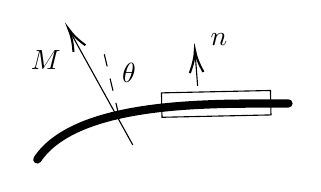
\begin{tikzpicture}[x=0.75pt,y=0.75pt,yscale=-1,xscale=1]
            %uncomment if require: \path (0,300); %set diagram left start at 0, and has height of 300

            %Shape: Free Drawing [id:dp47331539974666015] 
            \draw  [line width=3] [line join = round][line cap = round] (37.71,159.05) .. controls (58,128.62) and (132.31,132.55) .. (158.71,132.05) ;
            %Straight Lines [id:da5704698220523539] 
            \draw    (83.71,152.05) -- (53.68,97.8) ;
            \draw [shift={(52.71,96.05)}, rotate = 61.03] [color={rgb, 255:red, 0; green, 0; blue, 0 }  ][line width=0.75]    (10.93,-3.29) .. controls (6.95,-1.4) and (3.31,-0.3) .. (0,0) .. controls (3.31,0.3) and (6.95,1.4) .. (10.93,3.29)   ;
            %Shape: Rectangle [id:dp7424345376345918] 
            \draw   (97.52,126.96) -- (150.03,125.81) -- (150.29,137.58) -- (97.78,138.72) -- cycle ;
            %Straight Lines [id:da30639613261405896] 
            \draw  [dash pattern={on 4.5pt off 4.5pt}]  (76.95,137.58) -- (69.62,106.91) ;
            %Straight Lines [id:da2710244302735936] 
            \draw    (114.95,123.58) -- (113.77,108.24) ;
            \draw [shift={(113.62,106.24)}, rotate = 85.6] [color={rgb, 255:red, 0; green, 0; blue, 0 }  ][line width=0.75]    (10.93,-3.29) .. controls (6.95,-1.4) and (3.31,-0.3) .. (0,0) .. controls (3.31,0.3) and (6.95,1.4) .. (10.93,3.29)   ;

            % Text Node
            \draw (33.33,105.33) node [anchor=north west][inner sep=0.75pt]   [align=left] {$\displaystyle M$};
            % Text Node
            \draw (77.33,111.33) node [anchor=north west][inner sep=0.75pt]   [align=left] {$\displaystyle \theta $};
            % Text Node
            \draw (120,97.33) node [anchor=north west][inner sep=0.75pt]   [align=left] {$\displaystyle n$};


        \end{tikzpicture}

        \caption{磁化面电流}
    \end{figure}

    \begin{align}
        I' & - \mathbf{M} \times \mathrm{d} \mathbf{l}
    \end{align}

    磁化电流向里:
    \begin{align}
        \mathbf{i'} & = - \frac{ \mathbf{M} \cdot \mathrm{d} \mathbf{l}}{\mathrm{d} l} \\
                    & = - M \sin \theta                                                \\
                    & = \mathbf{M} \times \hat{\mathbf{n}}
    \end{align}

    \subsubsection{磁化体电流}

    \begin{figure}[ht]
        \centering


        \tikzset{every picture/.style={line width=0.75pt}} %set default line width to 0.75pt        

        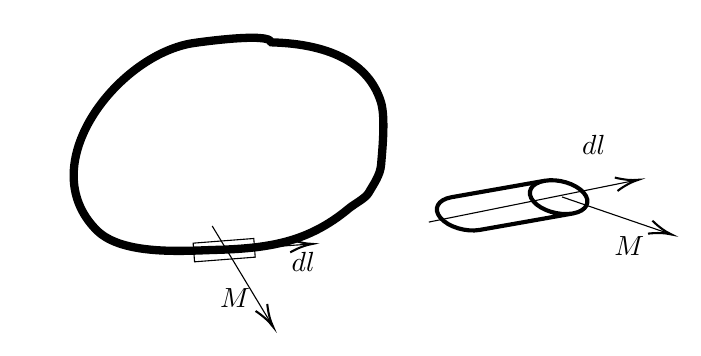
\begin{tikzpicture}[x=0.75pt,y=0.75pt,yscale=-1,xscale=1]
            %uncomment if require: \path (0,300); %set diagram left start at 0, and has height of 300

            %Shape: Free Drawing [id:dp08186547418424794] 
            \draw  [line width=3] [line join = round][line cap = round] (149.86,102.05) .. controls (149.86,96.96) and (113.78,102.13) .. (111.36,102.55) .. controls (75.58,108.87) and (34.59,161.29) .. (65.86,192.55) .. controls (78.19,204.89) and (108.43,202.43) .. (122.36,202.05) .. controls (148.53,201.34) and (167.54,198.57) .. (187.36,182.05) .. controls (190.07,179.79) and (195.34,177.18) .. (196.86,174.55) .. controls (199.32,170.29) and (202.46,165.96) .. (202.86,161.05) .. controls (203.3,155.51) and (205.11,138.57) .. (202.86,131.05) .. controls (196.15,108.7) and (172.05,102.64) .. (150.36,102.05) ;
            %Shape: Rectangle [id:dp5452653812131618] 
            \draw   (112.31,198.78) -- (141.53,196.53) -- (142.22,205.52) -- (113,207.77) -- cycle ;
            %Straight Lines [id:da8274796396425024] 
            \draw    (121.5,190.5) -- (149.82,237.41) ;
            \draw [shift={(150.86,239.12)}, rotate = 238.88] [color={rgb, 255:red, 0; green, 0; blue, 0 }  ][line width=0.75]    (10.93,-3.29) .. controls (6.95,-1.4) and (3.31,-0.3) .. (0,0) .. controls (3.31,0.3) and (6.95,1.4) .. (10.93,3.29)   ;
            %Straight Lines [id:da17878030773821108] 
            \draw    (127.27,202.15) -- (167.77,199.29) ;
            \draw [shift={(169.77,199.15)}, rotate = 175.96] [color={rgb, 255:red, 0; green, 0; blue, 0 }  ][line width=0.75]    (10.93,-3.29) .. controls (6.95,-1.4) and (3.31,-0.3) .. (0,0) .. controls (3.31,0.3) and (6.95,1.4) .. (10.93,3.29)   ;
            %Flowchart: Direct Access Storage [id:dp15709334846245548] 
            \draw  [line width=1.5]  (295.23,184.48) -- (250.43,192.39) .. controls (243.76,193.56) and (235.3,190.99) .. (231.53,186.65) .. controls (227.76,182.3) and (230.1,177.82) .. (236.77,176.65) -- (281.57,168.74)(300.47,174.48) .. controls (304.24,178.83) and (301.9,183.3) .. (295.23,184.48) .. controls (288.57,185.65) and (280.11,183.08) .. (276.34,178.74) .. controls (272.57,174.39) and (274.91,169.91) .. (281.57,168.74) .. controls (288.24,167.56) and (296.7,170.13) .. (300.47,174.48) ;
            %Straight Lines [id:da851886919377532] 
            \draw    (225.86,188.62) -- (324.88,168.63) ;
            \draw [shift={(326.84,168.24)}, rotate = 168.59] [color={rgb, 255:red, 0; green, 0; blue, 0 }  ][line width=0.75]    (10.93,-3.29) .. controls (6.95,-1.4) and (3.31,-0.3) .. (0,0) .. controls (3.31,0.3) and (6.95,1.4) .. (10.93,3.29)   ;
            %Straight Lines [id:da16988356011192574] 
            \draw    (290,176.5) -- (340.97,193.98) ;
            \draw [shift={(342.86,194.62)}, rotate = 198.93] [color={rgb, 255:red, 0; green, 0; blue, 0 }  ][line width=0.75]    (10.93,-3.29) .. controls (6.95,-1.4) and (3.31,-0.3) .. (0,0) .. controls (3.31,0.3) and (6.95,1.4) .. (10.93,3.29)   ;

            % Text Node
            \draw (124,219.5) node [anchor=north west][inner sep=0.75pt]   [align=left] {$\displaystyle M$};
            % Text Node
            \draw (158.5,202) node [anchor=north west][inner sep=0.75pt]   [align=left] {$\displaystyle dl$};
            % Text Node
            \draw (298.5,145.5) node [anchor=north west][inner sep=0.75pt]   [align=left] {$\displaystyle dl$};
            % Text Node
            \draw (314,194.5) node [anchor=north west][inner sep=0.75pt]   [align=left] {$\displaystyle M$};


        \end{tikzpicture}

        \caption{磁化体电流}
    \end{figure}

    考虑任一回路$L$,在$\mathrm{d} \mathbf{l}$处回路$L$套住的分子电流数目 $=$ 单位体积分子电流数目 $\times$ 小体积元体积。
    \begin{align}
        \int \mathbf{j'} \mathrm{d} \mathbf{S} & = I'                                            \\
                                               & = \oint I n \mathbf{S} \mathrm{d} \mathbf{l}    \\
                                               & = \oint \mathbf{M} \times \mathrm{d} \mathbf{l} \\
                                               & = \int \nabla \times \mathbf{M} \mathrm{d} S
    \end{align}

    从而:
    \begin{align}
        \mathbf{j'} & = \nabla \times \mathbf{M}
    \end{align}

    综上,磁介质会产生磁化面电流和磁化体电流:
    \begin{align}
        \mathbf{i'} & = \mathbf{M} \times \hat{\mathbf{n}} \\
        \mathbf{j'} & = \nabla \times \mathbf{M}
    \end{align}

    \section{磁介质中静磁场的基本定理}

    仿照电介质的基本方程,我们可以得到磁介质的基本方程。

    \subsection{磁介质的基本方程}

    \begin{align}
        \nabla \cdot \mathbf{B}  & = 0                                            \\
        \nabla \times \mathbf{B} & = \mu_0 (\mathbf{j}_\text{free} + \mathbf{j'})
    \end{align}

    第二个式子可以变形:
    \begin{align}
        \nabla \times \mathbf{B}                      & = \mu_0 \mathbf{j}_\text{free} + \mu_0 \nabla \times \mathbf{M} \\
        \nabla \times (\mathbf{B} - \mu_0 \mathbf{M}) & = \mu_0 \mathbf{j}_\text{free}
    \end{align}

    记磁场强度$\mathbf{H} = \mathbf{B} - \mu_0 \mathbf{M}$,则:
    \begin{align}
        \nabla \times \mathbf{H} & = \mu_0 \mathbf{j}_\text{free}
    \end{align}

    它们的积分形式是Gauss定理和环路定理:
    \begin{align}
        \oint \mathbf{B} \cdot \mathrm{d} \mathbf{S} & = 0                                                       \\
        \oint \mathbf{H} \cdot \mathrm{d} \mathbf{l} & = \int \mathbf{j}_\text{free} \cdot \mathrm{d} \mathbf{S}
    \end{align}

    \subsection{物质方程}

    对线性介质,有:
    \begin{align}
        \mathbf{M} & = \chi_m \mathbf{H}                                                              \\
        \mathbf{B} & = \mu_0 (\mathbf{H} + \mathbf{M}) = \mu_0 (1+\chi_m) \mathbf{H} = \mu \mathbf{H}
    \end{align}
    其中$\mu = \mu_0 (1+\chi_m)$为磁导率,$\chi_m$为磁化率。

    对于线性介质,当$\chi_m>0$时,磁介质为顺磁质;当$\chi_m<0$时,磁介质为抗磁质。

    非线性介质,磁化率$\chi_m$随磁场强度$\mathbf{H}$变化,磁导率大,有磁滞回线。例如铁磁质。自发磁化:原因是相邻原子之间电子的强的交换相互作用。

    Curie定律:顺磁质的磁化率$\chi_m$随温度$T$的变化关系:
    \begin{align}
        \chi_m & = \frac{N\mu_0m_0^2}{3kT} = \frac{C}{T}
    \end{align}
    其中$C$为与材料有关的常数。

    \begin{figure}[ht]
        \centering
        \includegraphics[width=10cm]{pic/6.2.2.png}
        \caption{磁介质的分类}
    \end{figure}

    \subsection{边值条件}

    同样的,在无传导电流的情况下,有:
    \begin{align}
        B_{1n} & =  B_{2n} \\
        H_{1t} & =  H_{2t}
    \end{align}

    \subsection{唯一性定理}

    同样的,我们也可以证明磁场有唯一性定理。

    \begin{example}
        (介质面与磁感应线重合)一圆环状磁介质与一无穷长直导线共轴,设磁介质磁导率$\mu$,直导线电流强度为$I$,求介质内外空间的磁感应强度的分布和介质表面的磁化面电流密度。

        由电流$I$和介质环的圆周对称,故知场$H$具有圆周对称,由电流$I$和介质环的平面对称性知$H$沿圆周方向$B$也沿圆周方向,因此介质面与磁感应线平行。

        介质内有:
        \begin{align}
            B_i & = \mu H = \mu \frac{I}{2\pi r}
        \end{align}

        介质外有:
        \begin{align}
            B_0 & = \mu_0 H = \frac{\mu_0 I}{2\pi r}
        \end{align}

        两个介质都在此处产生磁化面电流:
        \begin{align}
            i' & = (\mathbf{M}_i - \mathbf{M}_0) \times \hat{\mathbf{n}} \\
               & = \frac{B_i}{\mu_0} - \frac{B_0}{\mu_0}                 \\
               & = \frac{I}{2\pi\mu_0 r} (\mu - \mu_0)
        \end{align}
    \end{example}

    \begin{example}
        (介质界面与磁感应线垂直)在一同轴电缆(内半径$r_1$,外导体内半径$r_2$)中填满$\mu_1$和$\mu_2$两种介质各占一半空间且介质界面为通过电缆轴的平面。设通过电缆的电流强度$I_0$求介质中的磁场分布以及个质与导体毗连面上的面电流分布。

        观察垂直轴线的截面,计算感应面电流。

        传导电流$I_0$产生磁场$B_0$,$\mathbf{B}$垂直介质面,从而产生的$\mathbf{H}$垂直介质面。从而两个介质交界面无面电流密度。

        而在导体与介质交界面产生面电流与$I_0$沿一个方向,所以不改变磁感应强度的方向。在介质中:介质1和2界面处边界要求$B_{1n} = B_{2n}$,所以$B_1 = B_2=B$。

        则有环路定理:
        \begin{align}
            \frac{B}{\mu_1} \pi r + \frac{B}{\mu_2} \pi r & = I_0                                        \\
            B                                             & = \frac{\mu_1\mu_2 I_0}{\pi r (\mu_1+\mu_2)}
        \end{align}

        则介质1和介质2中磁场强度:
        \begin{align}
            H_1 & = \frac{B}{\mu_1} = \frac{\mu_2 I_0}{\pi r (\mu_1+\mu_2)} \\
            H_2 & = \frac{B}{\mu_2} = \frac{\mu_1 I_0}{\pi r (\mu_1+\mu_2)}
        \end{align}

        介质1和2中的磁化强度:
        \begin{align}
            M_1 & = \frac{B}{\mu_0} - H_1 = \frac{\mu_2 (\frac{\mu_1}{\mu_0}-1)I_0}{\pi r (\mu_1+\mu_2)} \\
            M_2 & = \frac{B}{\mu_0} - H_2 = \frac{\mu_1 (\frac{\mu_2}{\mu_0}-1)I_0}{\pi r (\mu_1+\mu_2)}
        \end{align}

        假设导体是理想导体,则$r<r_1$和$r>r_2$时$H=B=M=0$(就像理想导体内部的电场强度为0一样,可以用边值条件推出)。

        在$r=r_1$处感应面电流方向指向纸外与$\mathbf{I}$同向,在$r=r_2$处感应面电流方向指向纸外与$\mathbf{I}$反向。

        \begin{align}
            \mathbf{i'}_1|_{r=r_1} & = \frac{\mu_2 (\frac{\mu_1}{\mu_0}-1)I_0}{\pi r_1 (\mu_1+\mu_2)} \hat{\mathbf{n}}  \\
            \mathbf{i'}_1|_{r=r_2} & = -\frac{\mu_2 (\frac{\mu_1}{\mu_0}-1)I_0}{\pi r_2 (\mu_1+\mu_2)} \hat{\mathbf{n}} \\
            \mathbf{i'}_2|_{r=r_1} & = \frac{\mu_1 (\frac{\mu_2}{\mu_0}-1)I_0}{\pi r_1 (\mu_1+\mu_2)} \hat{\mathbf{n}}  \\
            \mathbf{i'}_2|_{r=r_2} & = -\frac{\mu_1 (\frac{\mu_2}{\mu_0}-1)I_0}{\pi r_2 (\mu_1+\mu_2)} \hat{\mathbf{n}}
        \end{align}

        我们现在再看沿着轴线的方向的自由面电流。

        取一个回路,导体中的磁场强度为0,有环路定理:
        \begin{align}
            H_i l        & = i_0 l                                 \\
            \mathbf{i}_0 & =  \mathbf{H}_i \times \hat{\mathbf{n}}
        \end{align}

        在$r=r_1$处$\mathbf{i}_0$与 $I$ 同向,$ r=r_2$处反向。

        \begin{align}
            \mathbf{i}_01|_{r=r_1} & = \frac{\mu_2 I_0}{\pi r_1 (\mu_1+\mu_2)} \hat{\mathbf{n}}  \\
            \mathbf{i}_01|_{r=r_2} & = -\frac{\mu_2 I_0}{\pi r_2 (\mu_1+\mu_2)} \hat{\mathbf{n}} \\
            \mathbf{i}_02|_{r=r_1} & = \frac{\mu_1 I_0}{\pi r_1 (\mu_1+\mu_2)} \hat{\mathbf{n}}  \\
            \mathbf{i}_02|_{r=r_2} & = -\frac{\mu_1 I_0}{\pi r_2 (\mu_1+\mu_2)} \hat{\mathbf{n}}
        \end{align}

        注意到:
        \begin{align}
            \mathbf{i'}_1|_{r=r_1} \pi r_1 + \mathbf{i'}_2|_{r=r_1} \pi r_1 & = I_0
        \end{align}

        从而电流只完全分布在表面,完全抗磁性。
    \end{example}

    \section{磁路定理}

    \subsection{电路定理与磁路定理}
    完全类比电路定理,电流对应磁通,电压对应磁势差,电阻对应磁阻。见下表:
    \begin{table}[ht]
        \centering
        \begin{tabular}{ccccc}
            \hline
            电路 & $\xi$        & $I$         & $R$                      & $\sigma$ \\
            磁路 & $\xi_m = NI$ & $\psi = BS$ & $R_m = \frac{ d}{\mu S}$ & $\mu$    \\ \hline
        \end{tabular}
        \caption{电路与磁路的对应}
    \end{table}

    \begin{table}[h!]
        \centering
        \begin{tabular}{ll}
            \hline
            \textbf{电路}                                                                                                          & \textbf{磁路}                                                                                                   \\
            \hline
            稳恒条件$\displaystyle \oint \mathbf{j} \cdot \mathrm{d}\mathbf{S} = 0$ \newline $\nabla \cdot \mathbf{j} = 0$           & Gauss定理$\displaystyle \oint \mathbf{B} \cdot \mathrm{d}\mathbf{S} = 0$ \newline $\nabla \cdot \mathbf{B} = 0$ \\
            Ohm定律 $\mathbf{j} = \sigma(\mathbf{E} + \mathbf{k}) = \sigma\mathbf{E}'$                                             & 物质方程 $\mathbf{B} = \mu\mathbf{H}$                                                                             \\
            电动势$\displaystyle \oint \mathbf{k} \cdot \mathrm{d}\mathbf{l} = \oint \mathbf{E}' \cdot \mathrm{d}d\mathbf{l} = \xi$ & $\displaystyle \oint \mathbf{H} \cdot \mathrm{d}\mathbf{l} = \sum I_0 = \xi_m$                                \\
            电导率$\sigma$的电流管                                                                                                      & 磁导率$\mu$的磁力线管                                                                                                 \\
            电流管电流强度 $I = \mathbf{j} \cdot \mathbf{S} = \text{const}$                                                             & 磁力线管磁通量 $\psi_B = \mathbf{B} \cdot \mathbf{S} = \text{const}$                                                 \\
            电阻 $R =\oint \frac{ \mathrm{d}\mathbf{l}}{\sigma\mathbf{S}}$                                                         & 磁阻 $R_m = \oint \frac{ \mathrm{d}\mathbf{l}}{\mu\mathbf{S}}$                                                  \\
            \hline
        \end{tabular}
        \caption{磁路定理}
    \end{table}

    \subsection{磁阻的串并联}

    和电阻一致。

    \subsection{磁路的方程}

    我们可以写出磁路的方程:
    \begin{align}
        \nabla \cdot \mathbf{B}  & = 0                                           \\
        \nabla \times \mathbf{H} & = 0                                           \\
        \mathbf{B}               & = \mu \mathbf{H}                              \\
        \psi_m                   & = \int \mathbf{B} \cdot \mathrm{d} \mathbf{S}
    \end{align}

    \subsection{Kirchhoff定律}

    \begin{align}
        \oint \frac{\mathbf{B}}{\mu} \cdot \mathrm{d} \mathbf{l} & = \sum \psi_i \oint \frac{ \mathrm{d} l}{\mu S} \\
                                                                 & = \sum \psi_iR_i                                \\
                                                                 & =\oint \mathbf{H} \cdot \mathrm{d} \mathbf{l}   \\
                                                                 & = nI = \sum \mathcal{E}
    \end{align}

    \section{磁荷法}

    无电荷的场有方程:
    \begin{align}
        \nabla \cdot \mathbf{D}  & = 0                                     \\
        \nabla \times \mathbf{E} & = 0                                     \\
        \mathbf{D}               & = \varepsilon_0 \mathbf{E} + \mathbf{P}
    \end{align}

    从而得到:
    \begin{align}
        \nabla \cdot \mathbf{E}  & = - \frac{\nabla \cdot  \mathbf{P}}{\varepsilon_0} = \frac{\rho'}{\varepsilon_0} \\
        \nabla \times \mathbf{E} & = 0                                                                              \\
        \sigma_e'                & = \mathbf{P} \cdot \hat{\mathbf{n}}
    \end{align}

    计算电容两极板的力:
    \begin{align}
        \frac{\mathbf{F}}{\Delta S} & = \frac{\sigma'_1 \sigma'_2}{2\varepsilon_0} \hat{\mathbf{n}}
    \end{align}

    类比地,无传导电流的场有方程:
    \begin{align}
        \nabla \cdot \mathbf{B}  & = 0                               \\
        \nabla \times \mathbf{H} & = 0                               \\
        \mathbf{B}               & = \mu_0 (\mathbf{H} + \mathbf{M})
    \end{align}

    从而得到:
    \begin{align}
        \nabla \cdot \mathbf{H}  & = - \nabla \cdot  \mathbf{M} = - \rho_m' \\
        \nabla \times \mathbf{H} & = 0                                      \\
        \mathbf{\sigma}_m'       & = \mathbf{M} \times \hat{\mathbf{n}}
    \end{align}

    可以计算两个磁荷之间的力:
    \begin{align}
        \frac{\mathbf{F}}{\Delta S} & = \frac{\mu_0\sigma_m1' \sigma_m2'}{2\mu_0} \hat{\mathbf{n}}
    \end{align}

    \begin{example}
        求两个均匀磁化,磁化强度为$M$的磁铁之间的引力


        \begin{align}
            \mathbf{F} = -\nabla W = -(\nabla w)V
        \end{align}
        其中$W$为能量密度,$V$为体积。

        磁场的能量密度:
        \begin{align}
            w = \frac{1}{2\mu_0}B^2 = \frac{\mu_0}{2} H^2
        \end{align}

        \begin{align}
            \mathbf{H}_{q_m} = \mathbf{H}_{\rho_m}V = \mathbf{H} (\nabla \cdot \vec{M} ) V
        \end{align}

        对比上面力的量纲,磁场感应力大小为:
        \begin{align}
            \mathbf{F} = \mu_0 \mathbf{H}_{q_m}
        \end{align}

        两个磁铁等效于两个平行板电容器极板间的力
        \begin{align}
            \mathbf{F}_e = \frac{\sigma_e}{2 \varepsilon_0} \sigma_e S = \frac{\sigma_e^2}{2 \varepsilon_0}S \quad \Longleftrightarrow \quad \mathbf{F}_m = \frac{\mu_0\sigma_m}{2} \sigma_m S = \frac{\mu_0 \sigma_m^2}{2} S
        \end{align}

        \begin{align}
            \sigma_m = \mathbf{M} \cdot \hat{\mathbf{n}} = M \quad \Rightarrow \quad \mathbf{F}_m = \frac{\mu_0 \sigma_m^2}{2} S = \frac{\mu_0 M^2}{2} S
        \end{align}
    \end{example}

    \chapter{电磁感应与磁能}

    \begin{block}{Faraday电磁感应定律}
        \begin{align}
            \mathcal{E} = - \frac{\mathrm{d} \psi}{\mathrm{d} t}
        \end{align}
    \end{block}

    \begin{block}{感应电场}
        \begin{align}
            \mathbf{E}_k = - \frac{\partial \mathbf{A}}{\partial t} + \mathbf{v} \times \mathbf{B}
        \end{align}
    \end{block}


    \begin{block}{似稳电路}
        \begin{align}
            \sum \mathcal{E} = \sum IR + \sum L \frac{\mathrm{d} I}{\mathrm{d} t} + \sum \frac{\int I(t) \mathrm{d} t}{C}
        \end{align}
    \end{block}

    \begin{block}{电感}
        \begin{align}
            \mathcal{E} & = - \frac{\mathrm{d} \phi}{\mathrm{d} t} =  - L \frac{\mathrm{d} I}{\mathrm{d} t} \\
            \psi        & = LI
        \end{align}
    \end{block}

    \begin{block}{磁能}
        \begin{align}
            W_m & = \frac{1}{2} \int \mathbf{B} \cdot \mathbf{H} \mathrm{d} V  \\
                & =  \frac{1}{2} \int\mathbf{j}_0 \cdot\mathbf{A} \mathrm{d} V \\
                & = \frac{1}{2} \sum \psi_i I_i                                \\
                & = \frac{1}{2} \sum L I^2
        \end{align}
        \begin{align}
            F & = (\nabla W)_\text{I不变}       \\
              & = (-\nabla W)_\text{$\psi$不变}
        \end{align}
    \end{block}

    \newpage

    \section{Faraday电磁感应定律}

    Faraday电磁感应定律又称“通量定律”:
    \begin{align}
        \mathcal{E} = - \frac{\mathrm{d} \psi}{\mathrm{d} t}
    \end{align}
    感应电动势的方向由Lenz定律给出。

    \subsection{感应电动势}

    感应电动势可以分为动生电动势和感生电动势:
    \begin{align}
        \mathcal{E} & = - \frac{\mathrm{d} \int \mathbf{B} \cdot \mathrm{d} \mathbf{S}}{\mathrm{d} t}                                                                           \\
                    & = - \frac{\mathrm{d} \int \mathbf{B} \cdot (\mathrm{d} \mathbf{l} \times \mathbf{v}\mathrm{d} t )}{\mathrm{d} t}                                          \\
                    & = - \int \frac{\partial}{\partial t}\mathbf{B} \cdot \mathrm{d} \mathbf{S}  + \oint \mathbf{v} \cdot \mathbf{B} \cdot\mathrm{d} \mathbf{l}                \\
                    & = - \int \nabla \times \frac{\partial\mathbf{A}}{\partial t} \cdot \mathrm{d} \mathbf{S}  + \oint \mathbf{v} \times \mathbf{B} \cdot\mathrm{d} \mathbf{l} \\
                    & = - \oint \frac{\partial\mathbf{A}}{\partial t} \cdot \mathrm{d} \mathbf{l}  + \oint \mathbf{v} \times \mathbf{B} \cdot\mathrm{d} \mathbf{l}
    \end{align}
    上式前面一项是感生电动势,后面一项是动生电动势。

    \begin{align}
        \oint  \mathbf{E}_k \cdot\mathrm{d} \mathbf{l} & = \mathcal{E}                                                                                                                          \\
                                                       & = - \oint \frac{\partial\mathbf{A}}{\partial t} \cdot \mathrm{d} \mathbf{l}  + \oint \mathbf{v} \cdot \mathbf{B} \mathrm{d} \mathbf{l}
    \end{align}

    \subsection{涡旋电场}

    产生的感应电场:
    \begin{align}
        \mathbf{E}_k & =\mathbf{E}_v+ \mathbf{E}_s                                              \\
                     & = - \frac{\partial\mathbf{A}}{\partial t} + \mathbf{v} \times \mathbf{B}
    \end{align}

    静电场满足的方程:
    \begin{align}
        \nabla \cdot \mathbf{E}_s  & = \frac{\rho}{\varepsilon_0} \\
        \nabla \times \mathbf{E}_s & = 0
    \end{align}


    涡旋电场满足的方程:
    \begin{align}
        \nabla \cdot \mathbf{E}_v  & = 0                                        \\
        \nabla \times \mathbf{E}_v & = - \frac{\partial \mathbf{B}}{\partial t}
    \end{align}

    积分形式有:
    \begin{align}
        \oint \mathbf{E}_v \cdot \mathrm{d} \mathbf{l} & = -  \int \frac{\partial\mathbf{B}}{\partial t} \cdot \mathrm{d} \mathbf{S}
    \end{align}

    这两者合起来就得到了Maxwell方程组中电场最终的式子:
    \begin{align}
        \nabla \cdot \mathbf{E}  & = \frac{\rho}{\varepsilon_0}               \\
        \nabla \times \mathbf{E} & = - \frac{\partial \mathbf{B}}{\partial t}
    \end{align}

    在电场中的电荷受到的力为:
    \begin{align}
        \mathbf{F} & = q (\mathbf{E}_s + \mathbf{v} \times \mathbf{B})
    \end{align}

    \begin{note}
        电源电动势来自于非静电力做功,将非静电能转换为电能,而Lorentz力不做功,怎么能转变为电能?

        但其分量$f_1$克服外力做负功,$f_2$非静电力做功转变为电能,因此总的物理过程是外力做功,通过Lorentz力转变为电能,Lorentz力并没有做功。
    \end{note}

    \section{互感和自感}

    \subsection{互感}

    考虑两个线圈,线圈2中有电流$I_2$,线圈2中的电流产生磁场,线圈1中的电流受到磁场力,从而产生感应电动势,这就是互感。

    \begin{figure}[ht]
        \centering
        \includegraphics[scale=0.2]{pic/7.2.1.png}
        \caption{互感}
    \end{figure}

    \begin{align}
        \psi_{12} & = \int \mathbf{B}_2 \cdot \mathrm{d} \mathbf{S}_1                                                      \\
                  & = \int \nabla \times \mathbf{A}_2 \cdot \mathrm{d} \mathbf{S}_1                                        \\
                  & = \oint \mathbf{A}_2 \cdot \mathrm{d} \mathbf{l}_1                                                     \\
                  & = \oint \oint \frac{\mu_0 I_2}{4\pi} \frac{\mathrm{d} \mathbf{l}_2 \cdot \mathrm{d} \mathbf{l}_1}{r^2} \\
                  & = L_{12} I_2
    \end{align}

    其中$M=L_{21}=L_{12}= \oint \oint \frac{\mu_0}{4\pi} \frac{\mathrm{d} \mathbf{l}_2 \cdot \mathrm{d} \mathbf{l}_1}{r^2}$为互感系数。单位是$H=Wb/A$。

    \subsection{自感}

    对于一个线圈的情况,线圈中有电流$I$,线圈中的电流产生磁场,线圈中的电流受到磁场力,从而产生感应电动势,这就是自感。

    \begin{align}
        \psi_{11} & = \int \mathbf{B}_1 \cdot \mathrm{d} \mathbf{S}_1                                                       \\
                  & = \int \nabla \times \mathbf{A}_1 \cdot \mathrm{d} \mathbf{S}_1                                         \\
                  & = \oint \mathbf{A}_1 \cdot \mathrm{d} \mathbf{l}_1                                                      \\
                  & = \oint \oint \frac{\mu_0 I_1}{4\pi} \frac{\mathrm{d} \mathbf{l}_1' \cdot \mathrm{d} \mathbf{l}_1}{r^2} \\
                  & = L_{11} I_1
    \end{align}

    其中$L=L_{11} = \oint \oint \frac{\mu_0}{4\pi} \frac{\mathrm{d} \mathbf{l}_1' \cdot \mathrm{d} \mathbf{l}_1}{r^2}$为自感系数。

    \subsection{电感}

    自感线圈可以作为电路元件。电感的电压电流关系为:
    \begin{align}
        \mathcal{E} & = - \frac{\mathrm{d} \psi}{\mathrm{d} t} = - L \frac{\mathrm{d} I}{\mathrm{d} t}
    \end{align}

    似稳电路中有Kirchhoff定律:
    \begin{align}
        \sum \mathcal{E} = \sum IR + \sum L \frac{\mathrm{d} I}{\mathrm{d} t} + \sum \frac{\int I(t) \mathrm{d} t}{C}
    \end{align}

    有下面LR、CR、LC电路:

    \subsubsection{LR电路}

    \begin{align}
        I(t) & = I_0 e^{-\frac{R}{L}t} \\
        \tau & = \frac{L}{R}
    \end{align}

    \subsubsection{CR电路}

    \begin{align}
        I(t) & = I_0 e^{-\frac{t}{RC}} \\
        \tau & = RC
    \end{align}

    \subsubsection{LC电路}

    根据Kirchhoff定律:
    \begin{align}
        L \frac{\mathrm{d} I}{\mathrm{d} t} + \frac{Q}{C}     & = 0 \\
        \frac{\mathrm{d}^2 Q}{\mathrm{d} t^2} + \frac{1}{LC}Q & = 0
    \end{align}

    这是一个振荡电路,解为:
    \begin{align}
        Q(t)   & = Q_0 \cos \omega t   \\
        \omega & = \frac{1}{\sqrt{LC}}
    \end{align}

    \subsection{电感的串并联}

    \subsubsection{串联}
    \begin{align}
        \mathcal{E}_1 & = - \frac{\mathrm{d} \psi_1}{\mathrm{d} t} = - \frac{\mathrm{d} (\psi_{11} + \psi_{12})}{\mathrm{d} t} = - (L_{11} + L_{12}) \frac{\mathrm{d} I}{\mathrm{d} t} \\
        \mathcal{E}_2 & = - \frac{\mathrm{d} \psi_2}{\mathrm{d} t} = - \frac{\mathrm{d} (\psi_{21} + \psi_{22})}{\mathrm{d} t} = - (L_{21} + L_{22}) \frac{\mathrm{d} I}{\mathrm{d} t}
    \end{align}

    而:
    \begin{align}
        \mathcal{E} = \mathcal{E}_1 +\mathcal{E}_2 = - (L_{11} + L_{12} + L_{21} + L_{22}) \frac{\mathrm{d} I}{\mathrm{d} t}
    \end{align}

    从而:
    \begin{align}
        L = L_{11} + L_{12} + L_{21} + L_{22}
    \end{align}

    若$L_{11}=L_{22}$。正接:如果完全耦合,则$L = 4L$;若完全不耦合,则$L = 2L$。反接:如果完全耦合,则$L = 0$;若完全不耦合,则$L = 2L$。

    \subsubsection{并联}

    \begin{align}
        \mathcal{E}_1 & = - \frac{\mathrm{d} \psi_1}{\mathrm{d} t} = - \frac{\mathrm{d} (\psi_{11} + \psi_{12})}{\mathrm{d} t} = - L_{11} \frac{\mathrm{d} I_1}{\mathrm{d} t}- L_{12} \frac{\mathrm{d} I_2}{\mathrm{d} t} \\
        \mathcal{E}_2 & = - \frac{\mathrm{d} \psi_2}{\mathrm{d} t} = - \frac{\mathrm{d} (\psi_{21} + \psi_{22})}{\mathrm{d} t} = - L_{21} \frac{\mathrm{d} I_1}{\mathrm{d} t}- L_{22} \frac{\mathrm{d} I_2}{\mathrm{d} t}
    \end{align}

    而:
    \begin{align}
        I           & = I_1 + I_2                                                            \\
        \mathcal{E} & = \mathcal{E}_1 =\mathcal{E}_2 = - L \frac{\mathrm{d} I}{\mathrm{d} t}
    \end{align}

    从而:
    \begin{align}
        L = \frac{L_{11}L_{22}-L_{12}^2}{L_{11}+L_{22}-2L_{12}}
    \end{align}

    \section{磁能}

    \subsection{$N$个载流线圈的磁能}

    考虑$N$个载流线圈由电流$I_i= 0$逐渐增大到$I_i$,计算该过程中电源对载流线圈所做的功,也就是载流线圈获得的磁能。

    \begin{align}
        \mathrm{d} W & = - \mathcal{E}_i \mathrm{d} q_i                                      \\
                     & = - \mathcal{E}_i I_i \mathrm{d} t                                    \\
                     & = - \frac{\mathrm{d}\sum_j  L_{ij} I_j}{\mathrm{d} t}I_i \mathrm{d} t \\
                     & = -\sum_j L_{ij} I_i\mathrm{d} I_j
    \end{align}

    从而,总的磁能为:
    \begin{align}
        \mathrm{d} W & = \frac{1}{2} \sum_{i,j} L_{ij} \mathrm{d}(I_i I_j)
    \end{align}

    \begin{align}
        W & = \frac{1}{2} \sum_{i,j} L_{ij} I_i I_j \\
          & = \frac{1}{2} \sum_{i} I_i\psi_i
    \end{align}

    \subsection{自能和互能}

    对两个线圈:
    \begin{align}
        W & = \frac{1}{2} L_{11} I_1^2 + \frac{1}{2} L_{22} I_2^2 + L_{12} I_1 I_2
    \end{align}

    自能是:
    \begin{align}
        W_1 & = \frac{1}{2} L_{11} I_1^2 \\
        W_2 & = \frac{1}{2} L_{22} I_2^2
    \end{align}

    互能,载流线圈在外场中的磁能:
    \begin{align}
        W_{12} & = L_{12} I_1 I_2 =  = \psi_{12} I_1 =  \mathbf{B}_2 \cdot I_1 \mathbf{S}_1 = \mathbf{B}_2 \cdot \mathbf{m}_1
    \end{align}

    \subsection{磁能和电能}

    \begin{align}
        W_e & = \int \frac{1}{2} \rho_0 \phi \mathrm{d} V = \frac{1}{2} \int \mathbf{E} \cdot \mathbf{D} \mathrm{d} V                  \\
        W_m & = \int \frac{1}{2} \mathbf{j}_0 \cdot\mathbf{A} \mathrm{d} V = \frac{1}{2} \int \mathbf{B} \cdot \mathbf{H} \mathrm{d} V
    \end{align}

    其中:
    \begin{align}
        \frac{1}{2} (\mathbf{j}_0 \cdot\mathbf{A}) (\mathrm{d} \mathbf{S} \cdot \mathrm{d} \mathbf{l}) & =\frac{1}{2}(\mathbf{A}\cdot\mathrm{d} \mathbf{l}) (\mathbf{j}_0\cdot \mathrm{d} \mathbf{S}  ) \\
                                                                                                       & =\frac{1}{2}\mathrm{d}I\cdot \mathrm{d}\psi
    \end{align}

    而:
    \begin{align}
        L & = \frac{\psi}{I} = \frac{nBS}{I} = \mu_0 n^2 S l = \mu_0 n^2 V
    \end{align}
    则有:
    \begin{align}
        W_m & = \frac{1}{2} LI^2                            \\
            & = \frac{1}{2}\mu_0 n^2 V                      \\
            & = \frac{1}{2}  \mathbf{B} \cdot \mathbf{H}  V
    \end{align}

    总结起来:
    \begin{align}
        W_m & = \frac{1}{2} \int \mathbf{B} \cdot \mathbf{H} \mathrm{d} V  \\
            & =  \frac{1}{2} \int\mathbf{j}_0 \cdot\mathbf{A} \mathrm{d} V \\
            & = \frac{1}{2} \sum \psi_i I_i                                \\
            & = \frac{1}{2} \sum L I^2
    \end{align}

    \chapter{电磁波}

    \begin{block}{Maxwell方程}
        \begin{align}
            \text{Maxwell方程} \quad
             & \left\{
            \begin{aligned}
                \nabla \cdot \mathbf{D}  & = \rho_0                                                \\
                \nabla \times \mathbf{E} & = - \frac{\partial \mathbf{B}}{\partial t}              \\
                \nabla \cdot \mathbf{B}  & = 0                                                     \\
                \nabla \times \mathbf{H} & = \mathbf{j}_0 + \frac{\partial \mathbf{D}}{\partial t}
            \end{aligned}
            \right.    \\
            \text{物质方程} \quad
             & \left\{
            \begin{aligned}
                \mathbf{D} & = \varepsilon_0 \mathbf{E} + \mathbf{P} \\
                \mathbf{B} & = \mu_0 (\mathbf{H} + \mathbf{M})
            \end{aligned}
            \right.    \\
            \text{边界条件} \quad
             & \left\{
            \begin{aligned}
                \hat{\mathbf{n}}\cdot(\mathbf{D}_1- \mathbf{D}_2)  & = \sigma_0     \\
                \hat{\mathbf{n}}\times(\mathbf{E}_1- \mathbf{E}_2) & = 0            \\
                \hat{\mathbf{n}}\cdot(\mathbf{B}_1- \mathbf{B}_2)  & = 0            \\
                \hat{\mathbf{n}}\times(\mathbf{H}_1- \mathbf{H}_2) & = \mathbf{j}_0
            \end{aligned}
            \right.
        \end{align}
    \end{block}

    \begin{block}{电磁波}
        \begin{align}
            \mathbf{k} \cdot \mathbf{B}  & = 0                                    \\
            \mathbf{k} \cdot \mathbf{D}  & = 0                                    \\
            \mathbf{k} \times \mathbf{E} & = \omega \mathbf{B}                    \\
            \mathbf{k} \times \mathbf{H} & = - \omega \mathbf{D}                  \\
            \frac{\omega}{k}             & = v = \frac{1}{\sqrt{\mu \varepsilon}}
        \end{align}
    \end{block}

    \begin{block}{能量}
        \begin{align}
            \text{能量密度} \quad
             &
            \begin{aligned}
                U & = \frac{1}{2} (\mathbf{H}\cdot \mathbf{B}+\mathbf{E}\cdot \mathbf{D}) = \mu \mathbf{H}\cdot \mathbf{H} = \varepsilon \mathbf{E}\cdot \mathbf{E}
            \end{aligned}
            \\
            \text{能流密度} \quad
             &
            \begin{aligned}
                \mathbf{S} & = \mathbf{E} \times \mathbf{H} = U \mathbf{v}
            \end{aligned}
            \\
            \text{动量密度} \quad
             &
            \begin{aligned}
                \mathbf{g} & = \frac{1}{v^2} \mathbf{S} = \mathbf{D} \times \mathbf{B}
            \end{aligned}
            \\
            \text{角动量密度} \quad
             &
            \begin{aligned}
                \mathbf{m} & = \mathbf{r} \times \mathbf{g}
            \end{aligned}
        \end{align}
    \end{block}


    \newpage

    \section{Pre Maxwell}

    在前面的章节,我们得到了在静电场、静磁场、电磁感应的方程:
    \begin{align}
        \nabla \cdot \mathbf{D}                                        & = \rho_0                                                                  \\
        \nabla \times \mathbf{E}                                       & = 0                                                                       \\
        \nabla \cdot \mathbf{B}                                        & = 0                                                                       \\
        \nabla \times \mathbf{H}                                       & = \mathbf{j}_0                                                            \\
        \frac{\partial \rho_0}{\partial t} + \nabla \cdot \mathbf{j}_0 & = 0                                                                       \\
        \mathbf{F}                                                     & = q(\mathbf{E} + \mathbf{v} \times \mathbf{B})                            \\
        \mathbf{D}                                                     & = \varepsilon_0 \mathbf{E} + \mathbf{P}                                   \\
        \mathbf{D}                                                     & = \varepsilon \mathbf{E}                                                  \\
        \mathbf{H}                                                     & = \frac{\mathbf{B}}{\mu_0} - \mathbf{M}                                   \\
        \mathbf{H}                                                     & = \frac{\mathbf{B}}{\mu}                                                  \\
        \mathbf{j}_0                                                   & = \sigma \mathbf{E}                                                       \\
        \mathbf{E}_k                                                   & = - \frac{\partial \mathbf{A}}{\partial t} + \mathbf{v} \times \mathbf{B}
    \end{align}

    现在我们把这些方程统一起来,得到Maxwell方程组。

    \section{Maxwell方程组}

    \subsection{两个推广}
    Maxwell给了两个推广:

    认为静电场中的:
    \begin{align}
        \nabla \cdot \mathbf{E} & = \frac{\rho}{\varepsilon_0} \\
        \nabla \cdot \mathbf{D} & = \rho_0
    \end{align}
    与
    \begin{align}
        \nabla \times \mathbf{B} & = 0
    \end{align}
    是普适的,这给出两个方程。

    \subsection{两个假设}
    Maxwell给了两个假设:

    \subsubsection{涡旋电场}

    \begin{align}
        \int \nabla \times \mathbf{E} \cdot \mathrm{d} \mathbf{S} & = \oint \mathbf{E} \cdot \mathrm{d} \mathbf{l} = - \int \frac{\partial}{\partial t}  \mathbf{B} \cdot \mathrm{d} \mathbf{S} \\
        \nabla \times \mathbf{E}                                  & = - \frac{\partial \mathbf{B}}{\partial t}
    \end{align}

    我们认为电场分为静电场和涡旋电场:
    \begin{align}
        \mathbf{E} & = \mathbf{E}_s + \mathbf{E}_v
    \end{align}

    则有两个方程:
    \begin{align}
        \nabla \cdot \mathbf{E}  & = \frac{\rho}{\varepsilon_0}               \\
        \nabla \times \mathbf{E} & = - \frac{\partial \mathbf{B}}{\partial t}
    \end{align}

    \subsubsection{位移电流}

    根据电荷守恒定律:
    \begin{align}
        \nabla \cdot \mathbf{j} + \frac{\partial \rho_0}{\partial t} & = 0      \\
        \nabla \cdot \mathbf{D}                                      & = \rho_0
    \end{align}
    有:
    \begin{align}
        \nabla \cdot \mathbf{j}_0                                  + \nabla \cdot \frac{\partial \mathbf{D}}{\partial t} = 0
    \end{align}
    我们认为位移电流是:
    \begin{align}
        \mathbf{j}_d & = \frac{\partial \mathbf{D}}{\partial t}
    \end{align}

    我们认为电流分为传导电流和位移电流:
    \begin{align}
        \mathbf{j} & = \mathbf{j}_0 + \frac{\partial \mathbf{D}}{\partial t}
    \end{align}

    \begin{align}
        \int \nabla \times \mathbf{H} \cdot \mathrm{d} \mathbf{S} & = \oint \mathbf{H} \cdot \mathrm{d} \mathbf{l} = \int \mathbf{j}_0 \cdot \mathrm{d} \mathbf{S} + \int \frac{\partial}{\partial t}  \mathbf{D} \cdot \mathrm{d} \mathbf{S} \\
        \nabla \times \mathbf{H}                                  & = \mathbf{j}_0 + \frac{\partial \mathbf{D}}{\partial t}
    \end{align}

    我们观察位移电流:
    \begin{align}
        \mathbf{j}_d & = \frac{\partial \mathbf{D}}{\partial t} = \frac{\partial (\varepsilon_0 \mathbf{E} + \mathbf{P})}{\partial t}
                     & = \varepsilon_0 \frac{\partial \mathbf{E}}{\partial t} + \frac{\partial \mathbf{P}}{\partial t}
                     & = \varepsilon_0 \frac{\partial \mathbf{E}}{\partial t} + \mathbf{j}_p
    \end{align}
    其中$\mathbf{j}_p$为极化电流。

    修正后的方程是:
    \begin{align}
        \nabla \times \mathbf{H} & = \mathbf{j}_0 + \frac{\partial \mathbf{D}}{\partial t}                                                                                                                                        \\
        \nabla \times \mathbf{B} & =\nabla \times \mu_0(\mathbf{H} + \mathbf{M}) = \mu_0 (\mathbf{j}_0 + \varepsilon_0 \frac{\partial \mathbf{E}}{\partial t} + \frac{\partial \mathbf{P}}{\partial t} + \nabla \times\mathbf{M})
    \end{align}

    \subsection{Maxwell方程组}
    现在我们得到了完整的Maxwell方程组:
    \begin{align}
        \nabla \cdot \mathbf{D}  & = \rho_0                                                \\
        \nabla \times \mathbf{E} & = - \frac{\partial \mathbf{B}}{\partial t}              \\
        \nabla \cdot \mathbf{B}  & = 0                                                     \\
        \nabla \times \mathbf{H} & = \mathbf{j}_0 + \frac{\partial \mathbf{D}}{\partial t}
    \end{align}

    物质方程:
    \begin{align}
        \mathbf{D} & = \varepsilon_0 \mathbf{E} + \mathbf{P} \\
        \mathbf{B} & = \mu_0 (\mathbf{H} + \mathbf{M})
    \end{align}

    边界条件:
    \begin{align}
        \hat{\mathbf{n}}\cdot(\mathbf{D}_1- \mathbf{D}_2)  & = \sigma_0     \\
        \hat{\mathbf{n}}\times(\mathbf{E}_1- \mathbf{E}_2) & = 0            \\
        \hat{\mathbf{n}}\cdot(\mathbf{B}_1- \mathbf{B}_2)  & = 0            \\
        \hat{\mathbf{n}}\times(\mathbf{H}_1- \mathbf{H}_2) & = \mathbf{j}_0
    \end{align}

    \section{电磁波}

    \subsection{电磁波的方程}
    根据Maxwell方程组,在真空中:
    \begin{align}
        \nabla \cdot \mathbf{E}  & = 0                                                          \\
        \nabla \times \mathbf{E} & = - \frac{\partial \mathbf{B}}{\partial t}                   \\
        \nabla \cdot \mathbf{B}  & = 0                                                          \\
        \nabla \times \mathbf{B} & = \mu_0 \varepsilon_0 \frac{\partial \mathbf{E}}{\partial t}
    \end{align}

    有:
    \begin{align}
        - \mu_0 \varepsilon_0 \frac{\partial^2}{\partial t^2} \mathbf{E} & = \nabla \times (\nabla \times \mathbf{E})               \\
                                                                         & = \nabla (\nabla \cdot \mathbf{E}) - \nabla^2 \mathbf{E} \\
                                                                         & = - \nabla^2 \mathbf{E}
    \end{align}

    得到:
    \begin{align}
        (\nabla^2  - \mu_0 \varepsilon_0 \frac{\partial^2}{\partial t^2})\mathbf{E} = 0
    \end{align}
    是典型的波动方程。

    可以得到真空中的光速:
    \begin{align}
        c = \frac{1}{\sqrt{\mu_0 \varepsilon_0}}
    \end{align}

    \subsection{波动方程的解}
    可以解出一维波动方程的解:
    \begin{align}
        \mathbf{E} = f(x - ct)+g(x + ct)
    \end{align}

    和平面波的解:
    \begin{align}
        \mathbf{E} = \mathbf{E}_0 e^{i ( \mathbf{k} \cdot \mathbf{r}-\omega t )}
    \end{align}

    \subsubsection{$\nabla \cdot \mathbf{E} = 0$}

    带入有:
    \begin{align}
        \nabla \cdot \mathbf{E} & = \partial_j (E_j e^{i ( \mathbf{k} \cdot \mathbf{r}-\omega t )}) \\
                                & = i k_j E_j e^{i ( \mathbf{k} \cdot \mathbf{r}-\omega t )}        \\
                                & = i \mathbf{k} \cdot \mathbf{E}                                   \\
                                & = 0
    \end{align}
    从而$\mathbf{k} \cdot \mathbf{E} = 0$,$\mathbf{E}$是一个横波。

    \subsubsection{$\nabla \cdot \mathbf{E} = 0$}

    同理:
    \begin{align}
        \mathbf{k} \cdot \mathbf{B} = 0
    \end{align}
$\mathbf{B}$是一个横波。

    \subsubsection{$\nabla \times \mathbf{E} = - \frac{\partial \mathbf{B}}{\partial t}$}

    带入有:
    \begin{align}
        \nabla \times \mathbf{E} & = \nabla \times (\mathbf{E}_0 e^{i ( \mathbf{k} \cdot \mathbf{r}-\omega t )})     \\
                                 & = i \mathbf{k} \times \mathbf{E}_0 e^{i ( \mathbf{k} \cdot \mathbf{r}-\omega t )} \\
                                 & = i \mathbf{k} \times \mathbf{E}                                                  \\
                                 & = - \frac{\partial \mathbf{B}}{\partial t}                                        \\
                                 & = - i \omega \mathbf{B}
    \end{align}

    从而有:
    \begin{align}
        \mathbf{k} \times \mathbf{E} = \omega \mathbf{B}
    \end{align}
    同相位,$\mathbf{E}$和$\mathbf{B}$垂直。

    \begin{align}
        k E & = \omega B
    \end{align}

    \subsubsection{$\nabla \times \mathbf{H} = \frac{\partial \mathbf{D}}{\partial t}$}

    同理有:
    \begin{align}
        \mathbf{k} \times \mathbf{H} = - \omega \mathbf{D}
    \end{align}

    有:
    \begin{align}
        k \frac{B}{\mu}  & = \omega \varepsilon E                 \\
        \frac{\omega}{k} & = v = \frac{1}{\sqrt{\mu \varepsilon}}
    \end{align}

    折射率:
    \begin{align}
        n = \frac{c}{v} = \sqrt{\mu_r \varepsilon_r} \sim \sqrt{\varepsilon_r}
    \end{align}

    \section{能流}

    \subsection{电荷守恒}

    由Maxwell方程组直接推出:
    \begin{align}
        \frac{\partial \rho_0}{\partial t} + \nabla \cdot \mathbf{j}_0 = 0
    \end{align}

    \subsection{能量守恒}

    同样有能量守恒:
    \begin{align}
        - \frac{\partial U}{\partial t} & = \nabla \cdot \mathbf{S} + \mathbf{j}_0 \cdot \mathbf{E} \\
        \text{能量密度的减少}                  & = \text{能量流出} + \text{对介质做功}
    \end{align}

    做功的表达式为:
    \begin{align}
        \mathbf{E}\cdot \mathbf{j}_0 & = \mathbf{E}\cdot (\nabla \times \mathbf{H} - \frac{\partial \mathbf{D}}{\partial t})                                                                        \\
                                     & = \nabla\cdot (\mathbf{E} \times \mathbf{H})+\mathbf{H}\cdot (\nabla \times \mathbf{E})  - \mathbf{E}\cdot \frac{\partial \mathbf{D}}{\partial t}            \\
                                     & = \nabla\cdot (\mathbf{E} \times \mathbf{H}) - \mathbf{H}\cdot \frac{\partial \mathbf{B}}{\partial t}-\mathbf{E}\cdot \frac{\partial \mathbf{D}}{\partial t} \\
                                     & = \nabla\cdot (\mathbf{E} \times \mathbf{H}) - \frac{1}{2}\frac{\partial}{\partial t} (\mathbf{H}\cdot \mathbf{B}+\mathbf{E}\cdot \mathbf{D})
    \end{align}

    与上面的能量守恒式对比,得到:
    \begin{align}
        \mathbf{S} & = \mathbf{E} \times \mathbf{H}                                        \\
        U          & = \frac{1}{2} (\mathbf{H}\cdot \mathbf{B}+\mathbf{E}\cdot \mathbf{D})
    \end{align}
    其中$\mathbf{S}$为能流密度(Poynting矢量),$U$为能量密度。

\subsection{能流密度}

能流密度:
\begin{align}
    \mathbf{S} & = \mathbf{E} \times \mathbf{H} = U \mathbf{v}
\end{align}

能量密度:
\begin{align}
    U & = \frac{1}{2} (\mathbf{H}\cdot \mathbf{B}+\mathbf{E}\cdot \mathbf{D}) = \mu \mathbf{H}\cdot \mathbf{H} = \varepsilon \mathbf{E}\cdot \mathbf{E}
\end{align}

动量密度:
\begin{align}
    \mathbf{g} & = \frac{1}{v^2} \mathbf{S} = \mathbf{D} \times \mathbf{B}
\end{align}

角动量密度:
\begin{align}
    \mathbf{m} & = \mathbf{r} \times \mathbf{g}
\end{align}


\end{document}

